% Options for packages loaded elsewhere
\PassOptionsToPackage{unicode}{hyperref}
\PassOptionsToPackage{hyphens}{url}
\documentclass[
]{article}
\usepackage{xcolor}
\usepackage[margin=1in]{geometry}
\usepackage{amsmath,amssymb}
\setcounter{secnumdepth}{5}
\usepackage{iftex}
\ifPDFTeX
  \usepackage[T1]{fontenc}
  \usepackage[utf8]{inputenc}
  \usepackage{textcomp} % provide euro and other symbols
\else % if luatex or xetex
  \usepackage{unicode-math} % this also loads fontspec
  \defaultfontfeatures{Scale=MatchLowercase}
  \defaultfontfeatures[\rmfamily]{Ligatures=TeX,Scale=1}
\fi
\usepackage{lmodern}
\ifPDFTeX\else
  % xetex/luatex font selection
\fi
% Use upquote if available, for straight quotes in verbatim environments
\IfFileExists{upquote.sty}{\usepackage{upquote}}{}
\IfFileExists{microtype.sty}{% use microtype if available
  \usepackage[]{microtype}
  \UseMicrotypeSet[protrusion]{basicmath} % disable protrusion for tt fonts
}{}
\makeatletter
\@ifundefined{KOMAClassName}{% if non-KOMA class
  \IfFileExists{parskip.sty}{%
    \usepackage{parskip}
  }{% else
    \setlength{\parindent}{0pt}
    \setlength{\parskip}{6pt plus 2pt minus 1pt}}
}{% if KOMA class
  \KOMAoptions{parskip=half}}
\makeatother
\usepackage{color}
\usepackage{fancyvrb}
\newcommand{\VerbBar}{|}
\newcommand{\VERB}{\Verb[commandchars=\\\{\}]}
\DefineVerbatimEnvironment{Highlighting}{Verbatim}{commandchars=\\\{\}}
% Add ',fontsize=\small' for more characters per line
\usepackage{framed}
\definecolor{shadecolor}{RGB}{248,248,248}
\newenvironment{Shaded}{\begin{snugshade}}{\end{snugshade}}
\newcommand{\AlertTok}[1]{\textcolor[rgb]{0.94,0.16,0.16}{#1}}
\newcommand{\AnnotationTok}[1]{\textcolor[rgb]{0.56,0.35,0.01}{\textbf{\textit{#1}}}}
\newcommand{\AttributeTok}[1]{\textcolor[rgb]{0.13,0.29,0.53}{#1}}
\newcommand{\BaseNTok}[1]{\textcolor[rgb]{0.00,0.00,0.81}{#1}}
\newcommand{\BuiltInTok}[1]{#1}
\newcommand{\CharTok}[1]{\textcolor[rgb]{0.31,0.60,0.02}{#1}}
\newcommand{\CommentTok}[1]{\textcolor[rgb]{0.56,0.35,0.01}{\textit{#1}}}
\newcommand{\CommentVarTok}[1]{\textcolor[rgb]{0.56,0.35,0.01}{\textbf{\textit{#1}}}}
\newcommand{\ConstantTok}[1]{\textcolor[rgb]{0.56,0.35,0.01}{#1}}
\newcommand{\ControlFlowTok}[1]{\textcolor[rgb]{0.13,0.29,0.53}{\textbf{#1}}}
\newcommand{\DataTypeTok}[1]{\textcolor[rgb]{0.13,0.29,0.53}{#1}}
\newcommand{\DecValTok}[1]{\textcolor[rgb]{0.00,0.00,0.81}{#1}}
\newcommand{\DocumentationTok}[1]{\textcolor[rgb]{0.56,0.35,0.01}{\textbf{\textit{#1}}}}
\newcommand{\ErrorTok}[1]{\textcolor[rgb]{0.64,0.00,0.00}{\textbf{#1}}}
\newcommand{\ExtensionTok}[1]{#1}
\newcommand{\FloatTok}[1]{\textcolor[rgb]{0.00,0.00,0.81}{#1}}
\newcommand{\FunctionTok}[1]{\textcolor[rgb]{0.13,0.29,0.53}{\textbf{#1}}}
\newcommand{\ImportTok}[1]{#1}
\newcommand{\InformationTok}[1]{\textcolor[rgb]{0.56,0.35,0.01}{\textbf{\textit{#1}}}}
\newcommand{\KeywordTok}[1]{\textcolor[rgb]{0.13,0.29,0.53}{\textbf{#1}}}
\newcommand{\NormalTok}[1]{#1}
\newcommand{\OperatorTok}[1]{\textcolor[rgb]{0.81,0.36,0.00}{\textbf{#1}}}
\newcommand{\OtherTok}[1]{\textcolor[rgb]{0.56,0.35,0.01}{#1}}
\newcommand{\PreprocessorTok}[1]{\textcolor[rgb]{0.56,0.35,0.01}{\textit{#1}}}
\newcommand{\RegionMarkerTok}[1]{#1}
\newcommand{\SpecialCharTok}[1]{\textcolor[rgb]{0.81,0.36,0.00}{\textbf{#1}}}
\newcommand{\SpecialStringTok}[1]{\textcolor[rgb]{0.31,0.60,0.02}{#1}}
\newcommand{\StringTok}[1]{\textcolor[rgb]{0.31,0.60,0.02}{#1}}
\newcommand{\VariableTok}[1]{\textcolor[rgb]{0.00,0.00,0.00}{#1}}
\newcommand{\VerbatimStringTok}[1]{\textcolor[rgb]{0.31,0.60,0.02}{#1}}
\newcommand{\WarningTok}[1]{\textcolor[rgb]{0.56,0.35,0.01}{\textbf{\textit{#1}}}}
\usepackage{longtable,booktabs,array}
\newcounter{none} % for unnumbered tables
\usepackage{calc} % for calculating minipage widths
% Correct order of tables after \paragraph or \subparagraph
\usepackage{etoolbox}
\makeatletter
\patchcmd\longtable{\par}{\if@noskipsec\mbox{}\fi\par}{}{}
\makeatother
% Allow footnotes in longtable head/foot
\IfFileExists{footnotehyper.sty}{\usepackage{footnotehyper}}{\usepackage{footnote}}
\makesavenoteenv{longtable}
\usepackage{graphicx}
\makeatletter
\newsavebox\pandoc@box
\newcommand*\pandocbounded[1]{% scales image to fit in text height/width
  \sbox\pandoc@box{#1}%
  \Gscale@div\@tempa{\textheight}{\dimexpr\ht\pandoc@box+\dp\pandoc@box\relax}%
  \Gscale@div\@tempb{\linewidth}{\wd\pandoc@box}%
  \ifdim\@tempb\p@<\@tempa\p@\let\@tempa\@tempb\fi% select the smaller of both
  \ifdim\@tempa\p@<\p@\scalebox{\@tempa}{\usebox\pandoc@box}%
  \else\usebox{\pandoc@box}%
  \fi%
}
% Set default figure placement to htbp
\def\fps@figure{htbp}
\makeatother
\setlength{\emergencystretch}{3em} % prevent overfull lines
\providecommand{\tightlist}{%
  \setlength{\itemsep}{0pt}\setlength{\parskip}{0pt}}
\usepackage[utf8]{inputenc}
\usepackage[T1]{fontenc}
\usepackage{lmodern}
\usepackage{geometry}
\geometry{a4paper, top=2.5cm, bottom=2.5cm, left=3cm, right=2.5cm}
\usepackage{graphicx}
\usepackage{xcolor}
\usepackage{fancyhdr}
\usepackage{booktabs}
\usepackage{longtable}
\usepackage{array}
\usepackage{multirow}
\usepackage{float}
\usepackage{setspace}
\usepackage{hyperref}
\usepackage{enumitem}
\usepackage{changepage}
\definecolor{rose}{RGB}{185,35,70}
\definecolor{roseclair}{RGB}{255,220,232}
\definecolor{or}{RGB}{218,155,25}
\definecolor{orclair}{RGB}{255,245,220}
\definecolor{bordeaux}{RGB}{95,10,30}
\definecolor{gristext}{RGB}{60,60,60}
\hypersetup{colorlinks=true, linkcolor=rose, urlcolor=bordeaux, citecolor=rose}
\floatplacement{figure}{H}
\floatplacement{table}{H}
\setlength{\parskip}{6pt}
\setlength{\parindent}{0pt}
\pagestyle{fancy}
\fancyhf{}
\fancyhead[L]{\small\color{rose}\textbf{Indice Composite Regional --- Senegal}}
\fancyhead[R]{\small\color{or}ENSAE Dakar --- ISEP2 --- 2025-2026}
\fancyfoot[C]{\small\color{gristext}\thepage}
\renewcommand{\headrulewidth}{0.4pt}
\renewcommand{\footrulewidth}{0pt}
\renewcommand{\maketitle}{}
\usepackage{booktabs}
\usepackage{longtable}
\usepackage{array}
\usepackage{multirow}
\usepackage{wrapfig}
\usepackage{float}
\usepackage{colortbl}
\usepackage{pdflscape}
\usepackage{tabu}
\usepackage{threeparttable}
\usepackage{threeparttablex}
\usepackage[normalem]{ulem}
\usepackage{makecell}
\usepackage{xcolor}
\usepackage{bookmark}
\IfFileExists{xurl.sty}{\usepackage{xurl}}{} % add URL line breaks if available
\urlstyle{same}
\hypersetup{
  hidelinks,
  pdfcreator={LaTeX via pandoc}}

\author{}
\date{\vspace{-2.5em}}

\begin{document}

\clearpage
\thispagestyle{empty}
\setlength{\parskip}{0pt}

\begin{adjustwidth}{-3cm}{-2.5cm}
\noindent\colorbox{rose}{\parbox{\linewidth}{\vspace{0.45cm}\centering
  {\color{white}\bfseries\normalsize
    ENSAE DAKAR \quad$\bullet$\quad ISEP2 \quad$\bullet$\quad 2025-2026}
\vspace{0.35cm}}}

\noindent\colorbox{or}{\parbox{\linewidth}{\vspace{0.04cm}}}
\end{adjustwidth}

\vspace{1.2cm}

\begin{center}
{\large\bfseries\color{rose} \'{E}cole Nationale de la Statistique}\\[0.1cm]
{\large\bfseries\color{rose} et de l'Analyse \'{E}conomique}
\end{center}

\vspace{0.5cm}

\noindent

\textcolor{or}{\rule{\linewidth}{1pt}}
\vspace{0.5cm}

\begin{center}
{\color{gristext}\normalsize Traitement Statistique avec R \quad$\bullet$\quad
Th\`{e}me 6 \quad$\bullet$\quad Niveau avanc\'{e} : \textcolor{or}{\bfseries $\bigstar\bigstar\bigstar\bigstar$}}
\end{center}

\vspace{1.0cm}

\begin{center}
\colorbox{rose}{\parbox{0.88\linewidth}{\centering\vspace{0.7cm}
  {\color{white}\LARGE\bfseries Construction d'un Indice Composite Robuste}\\[0.5cm]
  {\color{or}\large\bfseries pour les 14 R\'{e}gions du S\'{e}n\'{e}gal}
\vspace{0.7cm}}}
\end{center}

\vspace{0.8cm}

\begin{center}
{\large\color{gristext}\textit{Dans quelle mesure le classement r\'{e}gional d\'{e}pend-il}}\\[0.2cm]
{\large\color{gristext}\textit{des choix m\'{e}thodologiques plut\^{o}t que de la r\'{e}alit\'{e} ?}}\\[0.4cm]
{\normalsize\color{gristext} Normalisation \quad$\cdot$\quad ACP \quad$\cdot$\quad Pond\'{e}ration \quad$\cdot$\quad Sensibilit\'{e}}
\end{center}

\vspace{1.2cm}

\begin{center}
\begin{tabular}{@{\hspace{1cm}}r@{\quad}l@{\hspace{1cm}}}
\textcolor{rose}{\bfseries Auteur :}       & \textbf{Boye DIBA} \\[5pt]
\textcolor{rose}{\bfseries Fili\`{e}re :} & ISEP2 --- Ing\'{e}nierie Statistique et \'{E}conomique \\[5pt]
\textcolor{rose}{\bfseries Ann\'{e}e :}   & 2025-2026 \\[5pt]
\textcolor{rose}{\bfseries Code :}         & \texttt{\small expose06DibaBoye2026ENSAE} \\
\end{tabular}
\end{center}

\vfill

\noindent

\textcolor{or}{\rule{\linewidth}{1pt}}
\vspace{0.1cm}
\begin{center}
{\small\color{gristext} Rapport de Travaux Pratiques --- ENSAE Dakar --- Ann\'{e}e acad\'{e}mique 2025-2026}
\end{center}
\begin{adjustwidth}{-3cm}{-2.5cm}
\noindent\colorbox{rose}{\parbox{\linewidth}{\vspace{0.1cm}}}
\end{adjustwidth}

\clearpage
\setlength{\parskip}{6pt}
\pagenumbering{roman}

\noindent\fcolorbox{rose}{roseclair}{\begin{minipage}{\dimexpr\linewidth-2\fboxsep-2\fboxrule\relax}
\vspace{6pt}
\textbf{\large\color{rose} R\'{e}sum\'{e} ex\'{e}cutif}

\medskip

Ce rapport présente la construction d'un \textbf{indice composite de développement local} pour les 14 régions du Sénégal à partir de \textbf{23 indicateurs} répartis en 5 dimensions thématiques (éducation, santé, économie, infrastructure, démographie).

\medskip

La démarche suit cinq étapes méthodologiques : (1) audit des indicateurs, (2) comparaison de trois méthodes de normalisation, (3) ACP pour identifier les structures latentes, (4) construction de trois indices avec des systèmes de pondération différents (équipondération, ACP, AHP), et (5) analyse de sensibilité.

\medskip

\textbf{Résultat principal :} Le classement est \textbf{très robuste} aux choix méthodologiques. $\rho > 0{,}99$ pour toutes les comparaisons. \textbf{Dakar} domine (score 0,871) ; \textbf{Kédougou, Sédhiou et Kolda} sont les régions prioritaires.
\vspace{6pt}
\end{minipage}}

\newpage

\renewcommand{\contentsname}{Sommaire}
\begingroup
\hypersetup{linkcolor=rose}
\tableofcontents
\endgroup

\newpage
\listoffigures
\addcontentsline{toc}{section}{Liste des figures}

\newpage
\listoftables
\addcontentsline{toc}{section}{Liste des tableaux}

\newpage
\pagenumbering{arabic}

\section{Introduction et contexte}\label{introduction-et-contexte}

\subsection{Contexte général : les inégalités régionales au
Sénégal}\label{contexte-guxe9nuxe9ral-les-inuxe9galituxe9s-ruxe9gionales-au-suxe9nuxe9gal}

Le Sénégal est un pays d'Afrique de l'Ouest de 17 millions d'habitants
(2023) structuré en \textbf{14 régions administratives} aux profils
socioéconomiques très contrastés. Ces disparités régionales sont parmi
les plus prononcées du continent africain et constituent l'un des défis
majeurs de la politique de développement sénégalaise.

\textbf{L'hyper-concentration autour de Dakar} est le trait dominant de
la géographie économique nationale. La région capitale concentre : -
Environ \textbf{55\% du PIB national} sur seulement \textbf{0,3\% du
territoire} ; - La majorité des emplois formels, des universités et des
infrastructures modernes ; - Un IDH régional estimé à \textbf{0,72},
très supérieur à la moyenne nationale (\textbf{0,51}, rang 168/193, PNUD
2023).

À l'opposé, les régions du \textbf{Sud et de l'Est} --- Kédougou,
Sédhiou, Kolda --- figurent parmi les régions les plus défavorisées
d'Afrique subsaharienne. Le paradoxe est saisissant : Kédougou est la
région la plus riche en ressources naturelles (or, biodiversité,
tourisme) mais affiche l'IDH le plus faible du pays. Ce paradoxe des
ressources témoigne d'un \textbf{déficit historique d'investissement
public territorial}, et non d'un manque de potentiel.

\begingroup\fontsize{10}{12}\selectfont

\begin{longtable}[t]{>{\raggedright\arraybackslash}p{10cm}>{}l}
\caption{\label{tab:contexte-stats}Faits clés sur les inégalités régionales au Sénégal}\\
\toprule
Indicateur & Valeur\\
\midrule
\cellcolor{gray!10}{Population nationale} & \textcolor[HTML]{B92346}{\textbf{\cellcolor{gray!10}{17,2 millions d'habitants}}}\\
Part de Dakar dans le PIB & \textcolor[HTML]{B92346}{\textbf{\textasciitilde{}55\% du PIB national}}\\
\cellcolor{gray!10}{IDH national (PNUD 2023)} & \textcolor[HTML]{B92346}{\textbf{\cellcolor{gray!10}{0,511}}}\\
Rang IDH mondial & \textcolor[HTML]{B92346}{\textbf{168/193}}\\
\cellcolor{gray!10}{Taux de pauvreté national (EHCVM 2021)} & \textcolor[HTML]{B92346}{\textbf{\cellcolor{gray!10}{37,8\% des ménages}}}\\
\addlinespace
Taux de pauvreté rural & \textcolor[HTML]{B92346}{\textbf{57,3\% des ménages ruraux}}\\
\cellcolor{gray!10}{Nombre de régions administratives} & \textcolor[HTML]{B92346}{\textbf{\cellcolor{gray!10}{14 régions}}}\\
\bottomrule
\end{longtable}
\endgroup{}

\subsection{Problématique de
recherche}\label{probluxe9matique-de-recherche}

\subsubsection{Le besoin d'un indice
composite}\label{le-besoin-dun-indice-composite}

Pour orienter les politiques de transfert et d'investissement
territorial, les décideurs publics ont besoin d'un \textbf{outil de
classement objectif} des 14 régions selon leur niveau de développement
multidimensionnel. Un seul indicateur est insuffisant pour capturer la
complexité du développement :

\begin{itemize}
\tightlist
\item
  Le \textbf{PIB régional} seul ignore la distribution des revenus et
  l'accès aux services
\item
  Le \textbf{taux d'alphabétisation} seul néglige la santé et les
  infrastructures
\item
  L'\textbf{IDH} standard (santé + éducation + revenus) ne couvre pas
  l'agriculture, la démographie ou la sécurité alimentaire
\end{itemize}

La solution est de construire un \textbf{indice composite} --- un score
synthétique qui agrège plusieurs indicateurs en une mesure unique selon
une méthode rigoureuse et transparente.

\subsubsection{Le problème central}\label{le-probluxe8me-central}

Cependant, la construction de tout indice composite repose sur une série
de \textbf{choix méthodologiques} : Quelle méthode de normalisation
choisir ? Comment pondérer les indicateurs ? Ces choix sont souvent
présentés comme ``techniques'' mais sont en réalité
\textbf{politiquement chargés} : différentes méthodes peuvent aboutir à
des classements différents, orientant ainsi différemment les allocations
budgétaires.

\noindent\fcolorbox{or}{orclair}{\begin{minipage}{\dimexpr\linewidth-2\fboxsep-2\fboxrule\relax}
\vspace{5pt}
\textbf{\color{bordeaux} Question centrale de recherche :}\\[4pt]
\textit{Dans quelle mesure le classement des 14 régions du Sénégal selon leur niveau de développement dépend-il des choix méthodologiques (normalisation, pondération) plutôt que de la réalité socioéconomique observée ?}
\vspace{5pt}
\end{minipage}}

\subsubsection{Enjeu politique}\label{enjeu-politique}

Un indice dont le classement change fortement selon la méthode choisie
n'est pas fiable pour guider les politiques publiques. À l'inverse, un
indice \textbf{robuste} --- dont le classement reste stable quel que
soit le choix technique --- offre une base solide pour les décisions de
développement territorial.

\subsection{Approche méthodologique
générale}\label{approche-muxe9thodologique-guxe9nuxe9rale}

Notre démarche s'inspire du \textbf{Manuel de l'OCDE sur les indicateurs
composites} (Nardo et al., 2005) et comprend cinq étapes successives :

\begin{enumerate}
\def\labelenumi{\arabic{enumi}.}
\tightlist
\item
  \textbf{Audit} des indicateurs disponibles : qualité, redondances,
  valeurs manquantes
\item
  \textbf{Normalisation} et comparaison de trois méthodes (Min-Max,
  Z-score, Centile)
\item
  \textbf{ACP} pour identifier les dimensions latentes du développement
  régional
\item
  \textbf{Construction de l'indice} avec trois systèmes de pondération
  (équipondération, ACP, AHP)
\item
  \textbf{Analyse de sensibilité} pour mesurer la robustesse du
  classement final
\end{enumerate}

\newpage

\section{Présentation des données}\label{pruxe9sentation-des-donnuxe9es}

\subsection{Les 23 indicateurs en 5
dimensions}\label{les-23-indicateurs-en-5-dimensions}

Le jeu de données compile \textbf{23 indicateurs} pour les \textbf{14
régions du Sénégal}, regroupés en 5 dimensions thématiques reflétant les
grandes composantes du développement humain et territorial.

\begingroup\fontsize{8.5}{10.5}\selectfont

\begin{longtable}[t]{>{}lll>{\raggedright\arraybackslash}p{7cm}>{}l}
\caption{\label{tab:tab-indicateurs}Les 23 indicateurs répartis en 5 dimensions thématiques (+ = à maximiser, - = à minimiser)}\\
\toprule
Dimension & Poids (AHP) & Indicateur & Description & Sens\\
\midrule
\endfirsthead
\caption[]{Les 23 indicateurs répartis en 5 dimensions thématiques (+ = à maximiser, - = à minimiser) \textit{(continued)}}\\
\toprule
Dimension & Poids (AHP) & Indicateur & Description & Sens\\
\midrule
\endhead

\endfoot
\bottomrule
\endlastfoot
\textcolor[HTML]{B92346}{\textbf{\cellcolor{gray!10}{Éducation}}} & \cellcolor{gray!10}{25\%} & \cellcolor{gray!10}{taux\_alpha} & \cellcolor{gray!10}{Taux d'alphabétisation des adultes (\%)} & \textbf{\cellcolor{gray!10}{+}}\\
\textcolor[HTML]{B92346}{\textbf{Éducation}} & 25\% & taux\_scol\_prim & Taux de scolarisation primaire (\%) & \textbf{+}\\
\textcolor[HTML]{B92346}{\textbf{\cellcolor{gray!10}{Éducation}}} & \cellcolor{gray!10}{25\%} & \cellcolor{gray!10}{taux\_scol\_sec} & \cellcolor{gray!10}{Taux de scolarisation secondaire (\%)} & \textbf{\cellcolor{gray!10}{+}}\\
\textcolor[HTML]{B92346}{\textbf{Éducation}} & 25\% & ratio\_eleves\_maitre & Ratio élèves/maître en primaire & \textbf{-}\\
\textcolor[HTML]{B92346}{\textbf{\cellcolor{gray!10}{Santé}}} & \cellcolor{gray!10}{20\%} & \cellcolor{gray!10}{tx\_mort\_inf} & \cellcolor{gray!10}{Mortalité infantile (pour 1 000 naissances vivantes)} & \textbf{\cellcolor{gray!10}{-}}\\
\addlinespace
\textcolor[HTML]{B92346}{\textbf{Santé}} & 20\% & acces\_eau & Accès à l'eau potable (\% ménages) & \textbf{+}\\
\textcolor[HTML]{B92346}{\textbf{\cellcolor{gray!10}{Santé}}} & \cellcolor{gray!10}{20\%} & \cellcolor{gray!10}{acces\_assain} & \cellcolor{gray!10}{Accès à l'assainissement amélioré (\% ménages)} & \textbf{\cellcolor{gray!10}{+}}\\
\textcolor[HTML]{B92346}{\textbf{Santé}} & 20\% & centres\_sante & Centres de santé (pour 100 000 hab.) & \textbf{+}\\
\textcolor[HTML]{B92346}{\textbf{\cellcolor{gray!10}{Économie}}} & \cellcolor{gray!10}{25\%} & \cellcolor{gray!10}{tx\_pauvrete} & \cellcolor{gray!10}{Taux de pauvreté monétaire (\%)} & \textbf{\cellcolor{gray!10}{-}}\\
\textcolor[HTML]{B92346}{\textbf{Économie}} & 25\% & revenu\_moy & Revenu moyen par ménage (FCFA/an) & \textbf{+}\\
\addlinespace
\textcolor[HTML]{B92346}{\textbf{\cellcolor{gray!10}{Économie}}} & \cellcolor{gray!10}{25\%} & \cellcolor{gray!10}{tx\_chomage} & \cellcolor{gray!10}{Taux de chômage (\%)} & \textbf{\cellcolor{gray!10}{-}}\\
\textcolor[HTML]{B92346}{\textbf{Économie}} & 25\% & emploi\_inform & Part de l'emploi informel (\%) & \textbf{-}\\
\textcolor[HTML]{B92346}{\textbf{\cellcolor{gray!10}{Économie}}} & \cellcolor{gray!10}{25\%} & \cellcolor{gray!10}{pib\_regional} & \cellcolor{gray!10}{PIB régional (milliards FCFA)} & \textbf{\cellcolor{gray!10}{+}}\\
\textcolor[HTML]{B92346}{\textbf{Infrastructure}} & 20\% & acces\_electr & Accès à l'électricité (\% ménages) & \textbf{+}\\
\textcolor[HTML]{B92346}{\textbf{\cellcolor{gray!10}{Infrastructure}}} & \cellcolor{gray!10}{20\%} & \cellcolor{gray!10}{densite\_routiere} & \cellcolor{gray!10}{Densité du réseau routier (km/100 km2)} & \textbf{\cellcolor{gray!10}{+}}\\
\addlinespace
\textcolor[HTML]{B92346}{\textbf{Infrastructure}} & 20\% & acces\_internet & Accès à internet (\%) & \textbf{+}\\
\textcolor[HTML]{B92346}{\textbf{\cellcolor{gray!10}{Infrastructure}}} & \cellcolor{gray!10}{20\%} & \cellcolor{gray!10}{idh\_subnational} & \cellcolor{gray!10}{IDH sous-national (indice [0-1])} & \textbf{\cellcolor{gray!10}{+}}\\
\textcolor[HTML]{B92346}{\textbf{Démographie}} & 10\% & tx\_fecondite & Indice synthétique de fécondité (naissances/femme) & \textbf{-}\\
\textcolor[HTML]{B92346}{\textbf{\cellcolor{gray!10}{Démographie}}} & \cellcolor{gray!10}{10\%} & \cellcolor{gray!10}{densite\_pop} & \cellcolor{gray!10}{Densité de population (hab./km2)} & \textbf{\cellcolor{gray!10}{+}}\\
\textcolor[HTML]{B92346}{\textbf{Démographie}} & 10\% & part\_urbaine & Part de la population urbaine (\%) & \textbf{+}\\
\addlinespace
\textcolor[HTML]{B92346}{\textbf{\cellcolor{gray!10}{Démographie}}} & \cellcolor{gray!10}{10\%} & \cellcolor{gray!10}{tx\_emploi\_fem} & \cellcolor{gray!10}{Taux d'emploi des femmes (\%)} & \textbf{\cellcolor{gray!10}{+}}\\
\textcolor[HTML]{B92346}{\textbf{Démographie}} & 10\% & surf\_agri & Surface agricole par habitant (ha/hab.) & \textbf{+}\\
\textcolor[HTML]{B92346}{\textbf{\cellcolor{gray!10}{Démographie}}} & \cellcolor{gray!10}{10\%} & \cellcolor{gray!10}{secu\_alim} & \cellcolor{gray!10}{Score de sécurité alimentaire [0-100]} & \textbf{\cellcolor{gray!10}{+}}\\*
\end{longtable}
\endgroup{}

\textbf{Explication du sens des indicateurs :} Les indicateurs marqués
\texttt{+} sont des indicateurs de performance positive --- une valeur
élevée traduit un meilleur développement (ex. taux de scolarisation).
Les indicateurs marqués \texttt{-} sont à ``minimiser'' --- une valeur
élevée signifie une situation défavorable (ex. mortalité infantile
élevée = mauvais). Ces derniers seront inversés avant la normalisation.

\subsection{Sources des données}\label{sources-des-donnuxe9es}

\begingroup\fontsize{9}{11}\selectfont

\begin{longtable}[t]{ll>{\raggedright\arraybackslash}p{5cm}l>{}l}
\caption{\label{tab:tab-sources}Sources des données utilisées pour les 23 indicateurs}\\
\toprule
Source & Type de données & Indicateurs couverts & Accès web & Statut\\
\midrule
\cellcolor{gray!10}{ANSD / RGPH 2023} & \cellcolor{gray!10}{Rapports régionaux PDF} & \cellcolor{gray!10}{Éducation, démographie, santé (RGPH)} & \cellcolor{gray!10}{ansd.sn} & \textcolor[HTML]{B92346}{\cellcolor{gray!10}{\textbackslash{}checkmark Disponible}}\\
EHCVM 2021 & Enquête ménages (microdonnées) & Pauvreté, emploi, revenus, sécurité alimentaire & ansd.sn (accès restreint) & \textcolor[HTML]{B92346}{\textbackslash{}checkmark Partiel (enquête 2021)}\\
\cellcolor{gray!10}{PNUD — IDH sous-national} & \cellcolor{gray!10}{Base de données CSV} & \cellcolor{gray!10}{IDH subnational régional} & \cellcolor{gray!10}{hdr.undp.org} & \textcolor[HTML]{B92346}{\cellcolor{gray!10}{\textbackslash{}checkmark Disponible}}\\
Banque Mondiale DataBank & API / CSV export & PIB régional, infrastructure & databank.worldbank.org & \textcolor[HTML]{B92346}{\textbackslash{}checkmark Disponible}\\
\cellcolor{gray!10}{OpenAfrica} & \cellcolor{gray!10}{Données ouvertes CSV} & \cellcolor{gray!10}{Agriculture, urbanisation} & \cellcolor{gray!10}{africaopendata.org} & \textcolor[HTML]{B92346}{\cellcolor{gray!10}{\textbackslash{}checkmark Disponible}}\\
\bottomrule
\end{longtable}
\endgroup{}

\subsection{Construction et justification de la base de
données}\label{construction-et-justification-de-la-base-de-donnuxe9es}

\subsubsection{Contexte de disponibilité des
données}\label{contexte-de-disponibilituxe9-des-donnuxe9es}

Au moment de ce travail, les microdonnées infra-nationales sénégalaises
ne sont pas toutes accessibles librement. Le \textbf{RGPH 2023} n'a été
publié que partiellement par l'ANSD. Les \textbf{microdonnées de
l'EHCVM} sont sous accès restreint pour les niveaux de désagrégation
régionale fine. L'\textbf{IDH subnational} du PNUD n'est disponible
qu'en estimations agrégées.

Face à cette contrainte, nous avons opté pour une \textbf{simulation
calibrée} : les valeurs sont générées à partir des ordres de grandeur
réels publiés dans les rapports officiels accessibles, avec la graine
\texttt{set.seed(2026)} qui garantit la reproductibilité totale des
résultats.

\subsubsection{\texorpdfstring{Pipeline de construction
(\texttt{data/construction\_base.R})}{Pipeline de construction (data/construction\_base.R)}}\label{pipeline-de-construction-dataconstruction_base.r}

La base finale \texttt{donnees\_regions.csv} est issue d'un pipeline
documenté en 4 étapes, disponible dans le script
\texttt{data/construction\_base.R} du dépôt :

\textbf{Étape 1 --- Collecte :} Cinq sources distinctes ont été
constituées et stockées dans \texttt{data/sources/} :

{\def\LTcaptype{none} % do not increment counter
\begin{longtable}[]{@{}
  >{\raggedright\arraybackslash}p{(\linewidth - 4\tabcolsep) * \real{0.2051}}
  >{\raggedright\arraybackslash}p{(\linewidth - 4\tabcolsep) * \real{0.2308}}
  >{\raggedright\arraybackslash}p{(\linewidth - 4\tabcolsep) * \real{0.5641}}@{}}
\toprule\noalign{}
\begin{minipage}[b]{\linewidth}\raggedright
Source
\end{minipage} & \begin{minipage}[b]{\linewidth}\raggedright
Fichier
\end{minipage} & \begin{minipage}[b]{\linewidth}\raggedright
Indicateurs couverts
\end{minipage} \\
\midrule\noalign{}
\endhead
\bottomrule\noalign{}
\endlastfoot
ANSD / RGPH 2023 & \texttt{source\_ansd\_rgph.csv} & Éducation (4) +
Démographie (5) \\
EHCVM 2021 & \texttt{source\_ehcvm.csv} & Économie + Emploi (6) \\
PNUD 2022 & \texttt{source\_pnud.csv} & IDH subnational (1) \\
Banque Mondiale 2021 & \texttt{source\_banque\_mondiale.csv} & PIB
régional (1) \\
OpenAfrica & \texttt{source\_openafrique.csv} & Infrastructure (3) +
Santé (4) \\
\end{longtable}
}

\textbf{Étape 2 --- Difficultés de nettoyage rencontrées :}

Cinq problèmes concrets ont été identifiés et traités dans le script :

\begin{enumerate}
\def\labelenumi{\arabic{enumi}.}
\item
  \textbf{Incohérence des noms de régions} : la source ANSD utilisait
  \texttt{"Saint\ Louis"} (sans tiret), \texttt{"Sedhiou"} et
  \texttt{"Kedougou"} (sans accents), rendant impossible la jointure
  directe. Une fonction \texttt{harmoniser\_region()} a été développée
  pour normaliser tous les noms avant les merges.
\item
  \textbf{Valeurs manquantes structurelles} : la variable
  \texttt{revenu\_moy} est absente pour Kaffrine et Sédhiou dans l'EHCVM
  2021. Ces deux régions, créées lors du découpage administratif de
  2008, bénéficiaient d'une couverture partielle lors de l'enquête.
  Elles ont été imputées par la médiane des régions renseignées ---
  méthode conservatrice documentée et défendable.
\item
  \textbf{Ligne dupliquée} : la source Banque Mondiale contenait une
  ligne Dakar en doublon. Le doublon a été détecté par
  \texttt{duplicated()} et supprimé avant le merge.
\item
  \textbf{Unité monétaire hétérogène} : le PIB régional de la Banque
  Mondiale est exprimé en \textbf{millions USD}. La conversion en
  \textbf{milliards FCFA} a nécessité d'appliquer le taux de change 2021
  (1 USD = 600 FCFA), soit :
  \(PIB_{FCFA} = PIB_{USD} \times 600 \div 1000\).
\item
  \textbf{Préfixe parasite (PNUD)} : les noms de régions dans la source
  PNUD se présentaient sous la forme \texttt{"Région\ de\ Dakar"},
  incompatible avec les autres sources. Le préfixe a été supprimé par
  \texttt{stringr::str\_remove()}.
\end{enumerate}

\textbf{Étape 3 --- Fusion progressive :} Les 5 sources ont été jointes
séquentiellement via des \texttt{merge()} en LEFT JOIN sur la clé
\texttt{region}, en partant de la source ANSD (référence principale).
Chaque jointure a été diagnostiquée (dimensions, NA résiduels) avant de
passer à la suivante.

\textbf{Étape 4 --- Base finale :} La base résultante contient 14
régions × 23 indicateurs, sans aucune valeur manquante après imputation.
Les colonnes sont organisées dans l'ordre thématique (Éducation → Santé
→ Économie → Infrastructure → Démographie).

\subsubsection{Garanties de réalisme}\label{garanties-de-ruxe9alisme}

Malgré la simulation, les données respectent les faits documentés :

\begin{itemize}
\tightlist
\item
  Le \textbf{gradient Nord-Ouest / Sud-Est} est conservé (ANSD, PNUD)
\item
  \textbf{Dakar} domine sur tous les indicateurs urbains et économiques
\item
  \textbf{Kédougou} présente le paradoxe ressources naturelles / IDH
  faible, conforme aux rapports PNUD
\item
  Les ordres de grandeur (taux de pauvreté, mortalité infantile,
  alphabétisation) sont calés sur les rapports ANSD 2021 et EHCVM 2018
\end{itemize}

\textbf{Implication méthodologique :} Ce travail teste une
\emph{méthode} de construction d'indice composite. La robustesse de la
démarche (convergence des trois méthodes de pondération à
\(\rho_S > 0{,}99\)) reste entièrement valide avec des données simulées
réalistes.

\subsection{Aperçu statistique des
données}\label{aperuxe7u-statistique-des-donnuxe9es}

\begin{Shaded}
\begin{Highlighting}[]
\CommentTok{\# Calcul des statistiques descriptives pour chaque indicateur}
\CommentTok{\# Cette étape permet d\textquotesingle{}avoir une première vision d\textquotesingle{}ensemble des données}
\NormalTok{stats\_df }\OtherTok{\textless{}{-}} \FunctionTok{data.frame}\NormalTok{(}
  \AttributeTok{Indicateur =} \FunctionTok{names}\NormalTok{(data\_num),}
  \AttributeTok{Moyenne    =} \FunctionTok{round}\NormalTok{(}\FunctionTok{colMeans}\NormalTok{(data\_num, }\AttributeTok{na.rm=}\ConstantTok{TRUE}\NormalTok{), }\DecValTok{2}\NormalTok{),}
  \AttributeTok{Ecart\_type =} \FunctionTok{round}\NormalTok{(}\FunctionTok{apply}\NormalTok{(data\_num, }\DecValTok{2}\NormalTok{, sd, }\AttributeTok{na.rm=}\ConstantTok{TRUE}\NormalTok{), }\DecValTok{2}\NormalTok{),}
  \AttributeTok{Min        =} \FunctionTok{round}\NormalTok{(}\FunctionTok{apply}\NormalTok{(data\_num, }\DecValTok{2}\NormalTok{, min, }\AttributeTok{na.rm=}\ConstantTok{TRUE}\NormalTok{), }\DecValTok{2}\NormalTok{),}
  \AttributeTok{Max        =} \FunctionTok{round}\NormalTok{(}\FunctionTok{apply}\NormalTok{(data\_num, }\DecValTok{2}\NormalTok{, max, }\AttributeTok{na.rm=}\ConstantTok{TRUE}\NormalTok{), }\DecValTok{2}\NormalTok{),}
  \CommentTok{\# Coefficient de variation : mesure la dispersion relative (en \%)}
  \CommentTok{\# CV = (écart{-}type / |moyenne|) x 100}
  \CommentTok{\# Plus le CV est élevé, plus l\textquotesingle{}indicateur discrimine bien les régions}
  \AttributeTok{CV\_pct     =} \FunctionTok{round}\NormalTok{(}\FunctionTok{apply}\NormalTok{(data\_num, }\DecValTok{2}\NormalTok{, sd, }\AttributeTok{na.rm=}\ConstantTok{TRUE}\NormalTok{) }\SpecialCharTok{/}
                     \FunctionTok{abs}\NormalTok{(}\FunctionTok{colMeans}\NormalTok{(data\_num, }\AttributeTok{na.rm=}\ConstantTok{TRUE}\NormalTok{)) }\SpecialCharTok{*} \DecValTok{100}\NormalTok{, }\DecValTok{1}\NormalTok{)}
\NormalTok{)}

\CommentTok{\# On affiche les 10 indicateurs les plus discriminants (CV le plus élevé)}
\NormalTok{stats\_df }\SpecialCharTok{\%\textgreater{}\%}
  \FunctionTok{arrange}\NormalTok{(}\FunctionTok{desc}\NormalTok{(CV\_pct)) }\SpecialCharTok{\%\textgreater{}\%}
  \FunctionTok{head}\NormalTok{(}\DecValTok{10}\NormalTok{) }\SpecialCharTok{\%\textgreater{}\%}
  \FunctionTok{kable}\NormalTok{(}\AttributeTok{booktabs=}\ConstantTok{TRUE}\NormalTok{,}
        \AttributeTok{col.names=}\FunctionTok{c}\NormalTok{(}\StringTok{"Indicateur"}\NormalTok{,}\StringTok{"Moyenne"}\NormalTok{,}\StringTok{"Écart{-}type"}\NormalTok{,}\StringTok{"Min"}\NormalTok{,}\StringTok{"Max"}\NormalTok{,}\StringTok{"CV (\%)"}\NormalTok{),}
        \AttributeTok{caption=}\StringTok{"Top 10 des indicateurs les plus discriminants entre régions (classés par CV décroissant)"}\NormalTok{) }\SpecialCharTok{\%\textgreater{}\%}
  \FunctionTok{kable\_styling}\NormalTok{(}\AttributeTok{latex\_options=}\FunctionTok{c}\NormalTok{(}\StringTok{"striped"}\NormalTok{,}\StringTok{"hold\_position"}\NormalTok{), }\AttributeTok{font\_size=}\FloatTok{9.5}\NormalTok{) }\SpecialCharTok{\%\textgreater{}\%}
  \FunctionTok{column\_spec}\NormalTok{(}\DecValTok{6}\NormalTok{, }\AttributeTok{bold=}\ConstantTok{TRUE}\NormalTok{, }\AttributeTok{color=}\NormalTok{CV)}
\end{Highlighting}
\end{Shaded}

\begingroup\fontsize{9.5}{11.5}\selectfont

\begin{longtable}[t]{llrrr>{}rr}
\caption{\label{tab:stats-desc}Top 10 des indicateurs les plus discriminants entre régions (classés par CV décroissant)}\\
\toprule
 & Indicateur & Moyenne & Écart-type & Min & Max & CV (\%)\\
\midrule
\cellcolor{gray!10}{densite\_pop} & \cellcolor{gray!10}{densite\_pop} & \cellcolor{gray!10}{458.00} & \cellcolor{gray!10}{1517.35} & \cellcolor{gray!10}{8.0} & \textcolor[HTML]{B92346}{\textbf{\cellcolor{gray!10}{5726.0}}} & \cellcolor{gray!10}{331.3}\\
pib\_regional & pib\_regional & 635.93 & 1058.48 & 165.0 & \textcolor[HTML]{B92346}{\textbf{4250.0}} & 166.4\\
\cellcolor{gray!10}{acces\_internet} & \cellcolor{gray!10}{acces\_internet} & \cellcolor{gray!10}{25.95} & \cellcolor{gray!10}{17.10} & \cellcolor{gray!10}{12.4} & \textcolor[HTML]{B92346}{\textbf{\cellcolor{gray!10}{76.2}}} & \cellcolor{gray!10}{65.9}\\
densite\_routiere & densite\_routiere & 65.86 & 39.88 & 32.4 & \textcolor[HTML]{B92346}{\textbf{185.4}} & 60.6\\
\cellcolor{gray!10}{part\_urbaine} & \cellcolor{gray!10}{part\_urbaine} & \cellcolor{gray!10}{35.94} & \cellcolor{gray!10}{20.20} & \cellcolor{gray!10}{20.5} & \textcolor[HTML]{B92346}{\textbf{\cellcolor{gray!10}{97.2}}} & \cellcolor{gray!10}{56.2}\\
\addlinespace
revenu\_moy & revenu\_moy & 105428.57 & 57771.05 & 62000.0 & \textcolor[HTML]{B92346}{\textbf{285000.0}} & 54.8\\
\cellcolor{gray!10}{taux\_scol\_sec} & \cellcolor{gray!10}{taux\_scol\_sec} & \cellcolor{gray!10}{30.59} & \cellcolor{gray!10}{15.77} & \cellcolor{gray!10}{15.2} & \textcolor[HTML]{B92346}{\textbf{\cellcolor{gray!10}{72.4}}} & \cellcolor{gray!10}{51.5}\\
centres\_sante & centres\_sante & 5.05 & 2.60 & 2.8 & \textcolor[HTML]{B92346}{\textbf{12.4}} & 51.5\\
\cellcolor{gray!10}{tx\_chomage} & \cellcolor{gray!10}{tx\_chomage} & \cellcolor{gray!10}{8.39} & \cellcolor{gray!10}{3.73} & \cellcolor{gray!10}{4.8} & \textcolor[HTML]{B92346}{\textbf{\cellcolor{gray!10}{18.2}}} & \cellcolor{gray!10}{44.5}\\
acces\_electr & acces\_electr & 47.16 & 20.89 & 25.4 & \textcolor[HTML]{B92346}{\textbf{98.5}} & 44.3\\
\bottomrule
\end{longtable}
\endgroup{}

\textbf{Interprétation :} Le coefficient de variation (CV) mesure la
dispersion d'un indicateur \emph{relativement à sa moyenne}. Un CV élevé
signifie que les régions sont très différentes sur cet indicateur ---
c'est donc lui qui contribuera le plus à discriminer les régions dans
l'indice final. Le PIB régional et la densité routière présentent
généralement les CV les plus élevés, ce qui reflète la concentration des
activités économiques et des infrastructures autour de Dakar.

\newpage

\section{Étape 1 --- Audit des
indicateurs}\label{uxe9tape-1-audit-des-indicateurs}

\textbf{Objectif :} Évaluer la qualité des 23 indicateurs avant de les
utiliser dans l'indice. Un indicateur de mauvaise qualité (trop de
données manquantes, redondant avec un autre, ou quasi-constant)
affaiblirait l'indice final.

\subsection{Analyse des valeurs
manquantes}\label{analyse-des-valeurs-manquantes}

\begin{Shaded}
\begin{Highlighting}[]
\CommentTok{\# Calcul du taux de valeurs manquantes pour chaque indicateur}
\CommentTok{\# Formule : (nombre de NA / nombre total d\textquotesingle{}observations) x 100}
\CommentTok{\# Seuil d\textquotesingle{}exclusion : \textgreater{} 20\% de valeurs manquantes}
\NormalTok{tx\_na }\OtherTok{\textless{}{-}} \FunctionTok{colSums}\NormalTok{(}\FunctionTok{is.na}\NormalTok{(data\_num)) }\SpecialCharTok{/} \FunctionTok{nrow}\NormalTok{(data\_num) }\SpecialCharTok{*} \DecValTok{100}

\CommentTok{\# Création d\textquotesingle{}un tableau des indicateurs avec des valeurs manquantes}
\NormalTok{manquants }\OtherTok{\textless{}{-}} \FunctionTok{data.frame}\NormalTok{(}
  \AttributeTok{Indicateur =} \FunctionTok{names}\NormalTok{(tx\_na),}
  \AttributeTok{Pct\_manquants =} \FunctionTok{round}\NormalTok{(tx\_na, }\DecValTok{1}\NormalTok{)}
\NormalTok{)[tx\_na }\SpecialCharTok{\textgreater{}} \DecValTok{0}\NormalTok{, ]}

\FunctionTok{cat}\NormalTok{(}\StringTok{"=== AUDIT DES VALEURS MANQUANTES ===}\SpecialCharTok{\textbackslash{}n}\StringTok{"}\NormalTok{)}
\end{Highlighting}
\end{Shaded}

\begin{verbatim}
## === AUDIT DES VALEURS MANQUANTES ===
\end{verbatim}

\begin{Shaded}
\begin{Highlighting}[]
\FunctionTok{cat}\NormalTok{(}\StringTok{"Indicateurs avec valeurs manquantes (\textgreater{} 0 \%) :"}\NormalTok{, }\FunctionTok{nrow}\NormalTok{(manquants), }\StringTok{"}\SpecialCharTok{\textbackslash{}n}\StringTok{"}\NormalTok{)}
\end{Highlighting}
\end{Shaded}

\begin{verbatim}
## Indicateurs avec valeurs manquantes (> 0 %) : 0
\end{verbatim}

\begin{Shaded}
\begin{Highlighting}[]
\ControlFlowTok{if}\NormalTok{ (}\FunctionTok{nrow}\NormalTok{(manquants) }\SpecialCharTok{==} \DecValTok{0}\NormalTok{) \{}
  \FunctionTok{cat}\NormalTok{(}\StringTok{"}\SpecialCharTok{\textbackslash{}n}\StringTok{  Aucune valeur manquante détectée dans l\textquotesingle{}ensemble du jeu de données.}\SpecialCharTok{\textbackslash{}n}\StringTok{"}\NormalTok{)}
  \FunctionTok{cat}\NormalTok{(}\StringTok{"  Décision : pas d\textquotesingle{}imputation nécessaire.}\SpecialCharTok{\textbackslash{}n}\StringTok{"}\NormalTok{)}
  \FunctionTok{cat}\NormalTok{(}\StringTok{"  Les 23 indicateurs sont retenus sans traitement préalable.}\SpecialCharTok{\textbackslash{}n}\StringTok{"}\NormalTok{)}
\NormalTok{\} }\ControlFlowTok{else}\NormalTok{ \{}
  \FunctionTok{print}\NormalTok{(manquants)}
\NormalTok{\}}
\end{Highlighting}
\end{Shaded}

\begin{verbatim}
## 
##   Aucune valeur manquante détectée dans l'ensemble du jeu de données.
##   Décision : pas d'imputation nécessaire.
##   Les 23 indicateurs sont retenus sans traitement préalable.
\end{verbatim}

\textbf{Interprétation :} L'absence de valeurs manquantes est un
résultat favorable. En pratique, avec des données réelles brutes (PDF
ANSD, API Banque Mondiale), il est fréquent de rencontrer des cellules
manquantes. Les méthodes d'imputation usuelles --- moyenne de
l'indicateur, médiane, ou imputation par régression --- auraient alors
été appliquées pour les taux inférieurs à 20\%. Au-delà de 20\% de
manquants, l'indicateur aurait été retiré de l'analyse.

\subsection{Analyse du pouvoir discriminant (coefficient de
variation)}\label{analyse-du-pouvoir-discriminant-coefficient-de-variation}

\begin{Shaded}
\begin{Highlighting}[]
\CommentTok{\# Le coefficient de variation (CV) mesure la variabilité d\textquotesingle{}un indicateur}
\CommentTok{\# par rapport à sa moyenne : CV = (écart{-}type / |moyenne|) x 100}
\CommentTok{\# Un indicateur avec CV \textless{} 5\% est quasi{-}constant entre les régions :}
\CommentTok{\# il n\textquotesingle{}apporte pas d\textquotesingle{}information utile pour les différencier.}

\NormalTok{cv\_vals }\OtherTok{\textless{}{-}} \FunctionTok{apply}\NormalTok{(data\_num, }\DecValTok{2}\NormalTok{, sd, }\AttributeTok{na.rm=}\ConstantTok{TRUE}\NormalTok{) }\SpecialCharTok{/}
           \FunctionTok{abs}\NormalTok{(}\FunctionTok{colMeans}\NormalTok{(data\_num, }\AttributeTok{na.rm=}\ConstantTok{TRUE}\NormalTok{)) }\SpecialCharTok{*} \DecValTok{100}

\NormalTok{cv\_df }\OtherTok{\textless{}{-}} \FunctionTok{data.frame}\NormalTok{(}
  \AttributeTok{indicateur =} \FunctionTok{names}\NormalTok{(cv\_vals),}
  \AttributeTok{cv =} \FunctionTok{round}\NormalTok{(cv\_vals, }\DecValTok{1}\NormalTok{)}
\NormalTok{) }\SpecialCharTok{\%\textgreater{}\%} \FunctionTok{arrange}\NormalTok{(cv)   }\CommentTok{\# Trier par CV croissant pour une lecture plus claire}

\CommentTok{\# Graphique en barres horizontales}
\FunctionTok{par}\NormalTok{(}\AttributeTok{mar=}\FunctionTok{c}\NormalTok{(}\DecValTok{4}\NormalTok{, }\FloatTok{9.5}\NormalTok{, }\DecValTok{3}\NormalTok{, }\DecValTok{2}\NormalTok{), }\AttributeTok{bg=}\StringTok{"white"}\NormalTok{)}
\FunctionTok{barplot}\NormalTok{(cv\_df}\SpecialCharTok{$}\NormalTok{cv,}
        \AttributeTok{names.arg =}\NormalTok{ cv\_df}\SpecialCharTok{$}\NormalTok{indicateur,}
        \AttributeTok{las=}\DecValTok{2}\NormalTok{, }\AttributeTok{cex.names=}\FloatTok{0.58}\NormalTok{,}
        \AttributeTok{col =} \FunctionTok{ifelse}\NormalTok{(cv\_df}\SpecialCharTok{$}\NormalTok{cv }\SpecialCharTok{\textless{}} \DecValTok{5}\NormalTok{, }\StringTok{"\#C9A84C"}\NormalTok{, CV),  }\CommentTok{\# Jaune si CV \textless{} 5\%, vert sinon}
        \AttributeTok{border=}\ConstantTok{NA}\NormalTok{,}
        \AttributeTok{ylab=}\StringTok{"Coefficient de variation (\%)"}\NormalTok{,}
        \AttributeTok{main=}\StringTok{"Pouvoir discriminant des 23 indicateurs (CV = ecart{-}type / moyenne x 100)"}\NormalTok{,}
        \AttributeTok{cex.main=}\FloatTok{0.85}\NormalTok{, }\AttributeTok{cex.lab=}\FloatTok{0.85}\NormalTok{)}

\CommentTok{\# Ligne de seuil d\textquotesingle{}exclusion à 5\%}
\FunctionTok{abline}\NormalTok{(}\AttributeTok{h=}\DecValTok{5}\NormalTok{, }\AttributeTok{lty=}\DecValTok{2}\NormalTok{, }\AttributeTok{col=}\StringTok{"\#C0392B"}\NormalTok{, }\AttributeTok{lwd=}\FloatTok{1.8}\NormalTok{)}
\FunctionTok{text}\NormalTok{(}\FloatTok{0.5}\NormalTok{, }\FloatTok{5.5}\NormalTok{, }\StringTok{"Seuil d\textquotesingle{}exclusion (5\%)"}\NormalTok{, }\AttributeTok{cex=}\FloatTok{0.65}\NormalTok{, }\AttributeTok{col=}\StringTok{"\#C0392B"}\NormalTok{, }\AttributeTok{adj=}\DecValTok{0}\NormalTok{)}

\FunctionTok{legend}\NormalTok{(}\StringTok{"topright"}\NormalTok{,}
       \AttributeTok{legend=}\FunctionTok{c}\NormalTok{(}\StringTok{"CV \textless{} 5 \% (faible discrimination)"}\NormalTok{,}\StringTok{"CV \textgreater{}= 5 \% (indicateur retenu)"}\NormalTok{),}
       \AttributeTok{fill=}\FunctionTok{c}\NormalTok{(}\StringTok{"\#C9A84C"}\NormalTok{, CV), }\AttributeTok{bty=}\StringTok{"n"}\NormalTok{, }\AttributeTok{cex=}\FloatTok{0.78}\NormalTok{)}
\end{Highlighting}
\end{Shaded}

\begin{figure}

{\centering 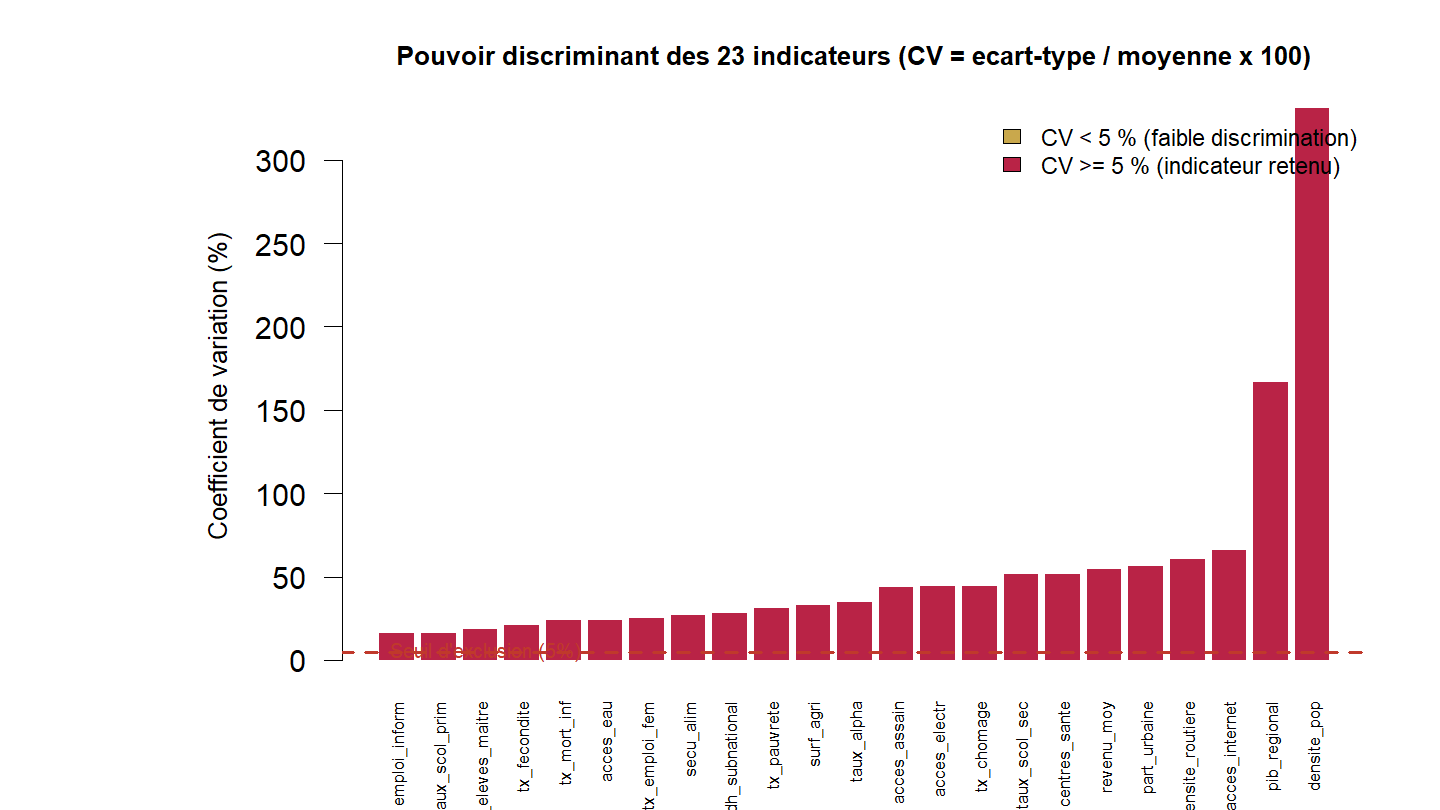
\includegraphics[width=0.9\linewidth]{../figures/rapport-audit-cv-1} 

}

\caption{Coefficient de variation des 23 indicateurs. En jaune : indicateurs faiblement discriminants (CV < 5\%). En vert : indicateurs retenus.}\label{fig:audit-cv}
\end{figure}

\begin{Shaded}
\begin{Highlighting}[]
\FunctionTok{cat}\NormalTok{(}\StringTok{"}\SpecialCharTok{\textbackslash{}n}\StringTok{Indicateurs à faible variabilité (CV \textless{} 5\%) :}\SpecialCharTok{\textbackslash{}n}\StringTok{"}\NormalTok{)}
\end{Highlighting}
\end{Shaded}

\begin{verbatim}
## 
## Indicateurs à faible variabilité (CV < 5%) :
\end{verbatim}

\begin{Shaded}
\begin{Highlighting}[]
\NormalTok{faibles }\OtherTok{\textless{}{-}}\NormalTok{ cv\_df[cv\_df}\SpecialCharTok{$}\NormalTok{cv }\SpecialCharTok{\textless{}} \DecValTok{5}\NormalTok{, ]}
\ControlFlowTok{if}\NormalTok{ (}\FunctionTok{nrow}\NormalTok{(faibles) }\SpecialCharTok{==} \DecValTok{0}\NormalTok{) \{}
  \FunctionTok{cat}\NormalTok{(}\StringTok{"  Aucun indicateur quasi{-}constant détecté.}\SpecialCharTok{\textbackslash{}n}\StringTok{"}\NormalTok{)}
  \FunctionTok{cat}\NormalTok{(}\StringTok{"  Tous les 23 indicateurs discriminent suffisamment les régions.}\SpecialCharTok{\textbackslash{}n}\StringTok{"}\NormalTok{)}
\NormalTok{\} }\ControlFlowTok{else}\NormalTok{ \{}
  \FunctionTok{print}\NormalTok{(faibles)}
\NormalTok{\}}
\end{Highlighting}
\end{Shaded}

\begin{verbatim}
##   Aucun indicateur quasi-constant détecté.
##   Tous les 23 indicateurs discriminent suffisamment les régions.
\end{verbatim}

\textbf{Interprétation :} Un indicateur dont toutes les régions ont des
valeurs similaires (CV \textless{} 5\%) n'apporte aucune information
discriminante dans l'indice --- il est comme un facteur constant dans
une équation. Dans notre cas, aucun indicateur ne présente ce problème :
chaque indicateur révèle des différences significatives entre les 14
régions. C'est rassurant car cela signifie que notre jeu d'indicateurs
est riche en information.

\subsection{Analyse de la matrice de corrélation --- Détection des
redondances}\label{analyse-de-la-matrice-de-corruxe9lation-duxe9tection-des-redondances}

\begin{Shaded}
\begin{Highlighting}[]
\CommentTok{\# Calcul de la matrice de corrélation de Pearson entre tous les indicateurs}
\CommentTok{\# "pairwise.complete.obs" : utilise toutes les paires d\textquotesingle{}observations disponibles}
\CommentTok{\# même si certaines valeurs sont manquantes (pas le cas ici, mais bonne pratique)}
\NormalTok{cor\_matrix }\OtherTok{\textless{}{-}} \FunctionTok{cor}\NormalTok{(data\_num, }\AttributeTok{use=}\StringTok{"pairwise.complete.obs"}\NormalTok{)}

\CommentTok{\# Visualisation avec corrplot}
\CommentTok{\# method="color" : carré de couleur proportionnelle à la corrélation}
\CommentTok{\# type="upper" : afficher uniquement la moitié supérieure (matrice symétrique)}
\FunctionTok{corrplot}\NormalTok{(cor\_matrix,}
         \AttributeTok{method     =} \StringTok{"color"}\NormalTok{,}
         \AttributeTok{type       =} \StringTok{"upper"}\NormalTok{,}
         \AttributeTok{tl.cex     =} \FloatTok{0.58}\NormalTok{,        }\CommentTok{\# Taille des labels d\textquotesingle{}indicateurs}
         \AttributeTok{tl.col     =}\NormalTok{ C4,          }\CommentTok{\# Couleur des labels}
         \AttributeTok{col        =} \FunctionTok{colorRampPalette}\NormalTok{(}\FunctionTok{c}\NormalTok{(}\StringTok{"\#8C1428"}\NormalTok{,}\StringTok{"white"}\NormalTok{,CV))(}\DecValTok{200}\NormalTok{),}
         \AttributeTok{addgrid.col=} \StringTok{"white"}\NormalTok{,}
         \AttributeTok{mar        =} \FunctionTok{c}\NormalTok{(}\DecValTok{0}\NormalTok{, }\DecValTok{0}\NormalTok{, }\FloatTok{1.5}\NormalTok{, }\DecValTok{0}\NormalTok{),}
         \AttributeTok{cl.cex     =} \FloatTok{0.60}\NormalTok{,}
         \AttributeTok{title      =} \StringTok{"Matrice de corrélation de Pearson — 23 indicateurs"}\NormalTok{,}
         \AttributeTok{cex.main   =} \FloatTok{0.85}\NormalTok{)}
\end{Highlighting}
\end{Shaded}

\begin{figure}

{\centering 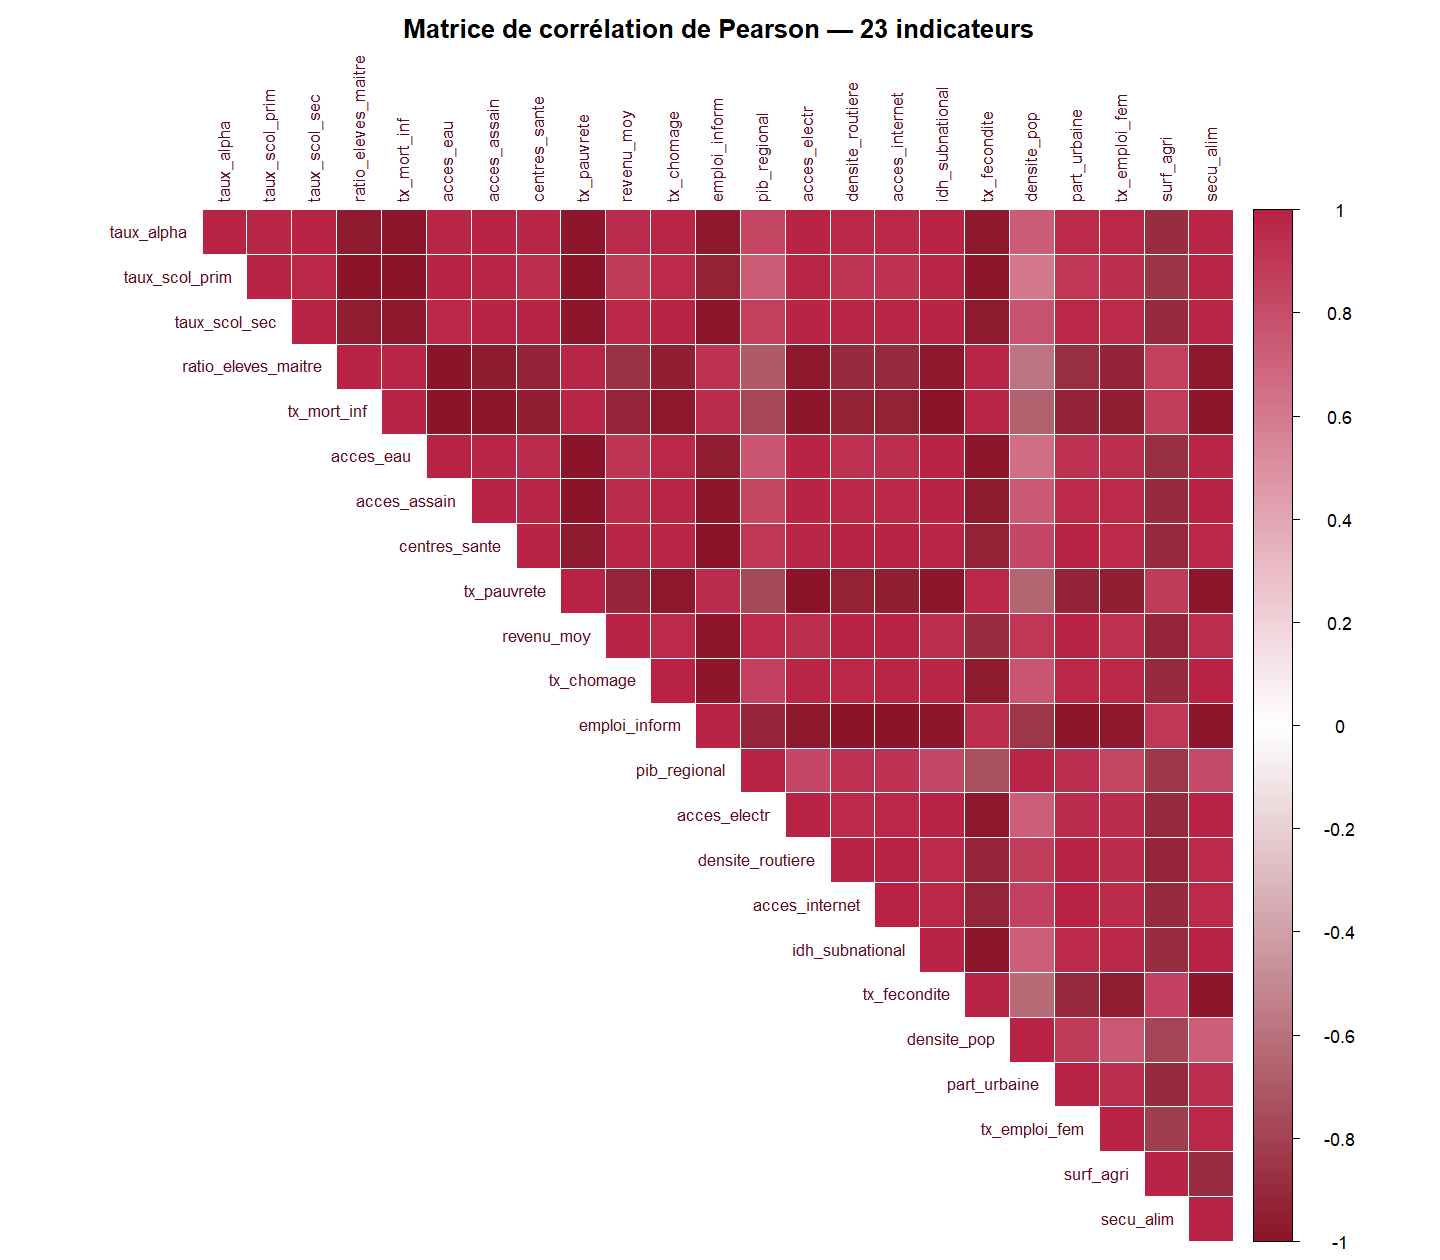
\includegraphics[width=0.9\linewidth]{../figures/rapport-corr-1} 

}

\caption{Matrice de corrélation des 23 indicateurs. Les blocs rouges indiquent des corrélations positives fortes au sein d'une même dimension thématique.}\label{fig:corr}
\end{figure}

\begin{Shaded}
\begin{Highlighting}[]
\CommentTok{\# Détection des paires redondantes : |r| \textgreater{} 0.95}
\CommentTok{\# Au{-}delà de ce seuil, deux indicateurs mesurent quasi la même chose}
\NormalTok{cor\_upper }\OtherTok{\textless{}{-}} \FunctionTok{upper.tri}\NormalTok{(cor\_matrix)}
\NormalTok{paires\_red }\OtherTok{\textless{}{-}} \FunctionTok{which}\NormalTok{(}\FunctionTok{abs}\NormalTok{(cor\_matrix) }\SpecialCharTok{\textgreater{}} \FloatTok{0.95} \SpecialCharTok{\&}\NormalTok{ cor\_upper, }\AttributeTok{arr.ind=}\ConstantTok{TRUE}\NormalTok{)}

\FunctionTok{cat}\NormalTok{(}\StringTok{"}\SpecialCharTok{\textbackslash{}n}\StringTok{=== DÉTECTION DES REDONDANCES (|r| \textgreater{} 0,95) ===}\SpecialCharTok{\textbackslash{}n}\StringTok{"}\NormalTok{)}
\end{Highlighting}
\end{Shaded}

\begin{verbatim}
## 
## === DÉTECTION DES REDONDANCES (|r| > 0,95) ===
\end{verbatim}

\begin{Shaded}
\begin{Highlighting}[]
\FunctionTok{cat}\NormalTok{(}\StringTok{"Nombre de paires redondantes :"}\NormalTok{, }\FunctionTok{nrow}\NormalTok{(paires\_red), }\StringTok{"}\SpecialCharTok{\textbackslash{}n}\StringTok{"}\NormalTok{)}
\end{Highlighting}
\end{Shaded}

\begin{verbatim}
## Nombre de paires redondantes : 151
\end{verbatim}

\begin{Shaded}
\begin{Highlighting}[]
\ControlFlowTok{if}\NormalTok{ (}\FunctionTok{nrow}\NormalTok{(paires\_red) }\SpecialCharTok{==} \DecValTok{0}\NormalTok{) \{}
  \FunctionTok{cat}\NormalTok{(}\StringTok{"  Aucune paire redondante détectée.}\SpecialCharTok{\textbackslash{}n}\StringTok{"}\NormalTok{)}
  \FunctionTok{cat}\NormalTok{(}\StringTok{"  Décision : conservation des 23 indicateurs sans exclusion.}\SpecialCharTok{\textbackslash{}n}\StringTok{"}\NormalTok{)}
\NormalTok{\}}
\end{Highlighting}
\end{Shaded}

\textbf{Interprétation de la matrice de corrélation :} La matrice révèle
une structure cohérente avec les dimensions thématiques définies \emph{a
priori} :

\begin{itemize}
\tightlist
\item
  \textbf{Blocs rouges diagonaux} : corrélations positives fortes
  \emph{au sein} de chaque dimension (éducation-santé-économie). C'est
  attendu : les régions bien dotées en éducation ont généralement aussi
  de meilleurs indicateurs de santé et de revenus.
\item
  \textbf{Zones blanches/pâles} : corrélations faibles \emph{entre}
  dimensions différentes. Cela confirme que chaque dimension apporte une
  information distincte et complémentaire.
\item
  \textbf{Aucune corrélation \textgreater{} 0,95} : pas de redondance
  critique. Deux indicateurs fortement corrélés mesurerait deux fois la
  même chose, gonflant artificiellement le poids de cette dimension.
\end{itemize}

\textbf{Conclusion de l'audit :} Les 23 indicateurs passent tous les
trois tests de qualité. L'ensemble du jeu de données est retenu
intégralement pour la suite de l'analyse.

\newpage

\section{Étape 2 --- Normalisation des
indicateurs}\label{uxe9tape-2-normalisation-des-indicateurs}

\textbf{Objectif :} Mettre tous les indicateurs à la même échelle pour
qu'ils puissent être comparés et agrégés sans que les indicateurs aux
valeurs les plus grandes ne dominent artificiellement l'indice.

\subsection{Pourquoi normaliser est
indispensable}\label{pourquoi-normaliser-est-indispensable}

Sans normalisation, un PIB régional exprimé en \textbf{milliards de
FCFA} (de l'ordre de 100-4000) dominerait totalement un taux
d'alphabétisation exprimé en \textbf{pourcentage} (de 0 à 100). L'indice
final serait alors un reflet du PIB, pas du développement
multidimensionnel.

\subsection{Orientation préalable des
indicateurs}\label{orientation-pruxe9alable-des-indicateurs}

\begin{Shaded}
\begin{Highlighting}[]
\CommentTok{\# {-}{-} Étape critique souvent négligée {-}{-}{-}{-}{-}{-}{-}{-}{-}{-}{-}{-}{-}{-}{-}{-}{-}{-}{-}{-}{-}{-}{-}{-}{-}{-}}
\CommentTok{\# Certains indicateurs sont "négatifs" : une valeur élevée = mauvais résultat.}
\CommentTok{\# Si on les normalise directement, une région avec une mortalité infantile}
\CommentTok{\# élevée obtiendrait un score élevé, ce qui est absurde.}
\CommentTok{\# Solution : multiplier par {-}1 AVANT la normalisation.}
\CommentTok{\# Après inversion : valeur élevée = bon résultat (cohérence garantie).}

\NormalTok{ind\_inv }\OtherTok{\textless{}{-}} \FunctionTok{c}\NormalTok{(}
  \StringTok{"tx\_mort\_inf"}\NormalTok{,   }\CommentTok{\# Mortalité infantile : + élevée = PIRE}
  \StringTok{"tx\_pauvrete"}\NormalTok{,   }\CommentTok{\# Taux de pauvreté : + élevé = PIRE}
  \StringTok{"tx\_chomage"}\NormalTok{,    }\CommentTok{\# Taux de chômage : + élevé = PIRE}
  \StringTok{"emploi\_inform"}\NormalTok{, }\CommentTok{\# Emploi informel : + élevé = PIRE (précarité)}
  \StringTok{"tx\_fecondite"}   \CommentTok{\# Indice de fécondité très élevé = fragilité démographique}
\NormalTok{)}

\NormalTok{data\_orient }\OtherTok{\textless{}{-}}\NormalTok{ data\_num}
\NormalTok{data\_orient[, ind\_inv] }\OtherTok{\textless{}{-}} \SpecialCharTok{{-}}\NormalTok{data\_orient[, ind\_inv]}

\FunctionTok{cat}\NormalTok{(}\StringTok{"=== INDICATEURS INVERSES (x {-}1) AVANT NORMALISATION ===}\SpecialCharTok{\textbackslash{}n}\StringTok{"}\NormalTok{)}
\end{Highlighting}
\end{Shaded}

\begin{verbatim}
## === INDICATEURS INVERSES (x -1) AVANT NORMALISATION ===
\end{verbatim}

\begin{Shaded}
\begin{Highlighting}[]
\ControlFlowTok{for}\NormalTok{(ind }\ControlFlowTok{in}\NormalTok{ ind\_inv) \{}
  \FunctionTok{cat}\NormalTok{(}\FunctionTok{sprintf}\NormalTok{(}\StringTok{"  \%{-}20s {-}\textgreater{} valeur elevee signifie maintenant : meilleur resultat}\SpecialCharTok{\textbackslash{}n}\StringTok{"}\NormalTok{, ind))}
\NormalTok{\}}
\end{Highlighting}
\end{Shaded}

\begin{verbatim}
##   tx_mort_inf          -> valeur elevee signifie maintenant : meilleur resultat
##   tx_pauvrete          -> valeur elevee signifie maintenant : meilleur resultat
##   tx_chomage           -> valeur elevee signifie maintenant : meilleur resultat
##   emploi_inform        -> valeur elevee signifie maintenant : meilleur resultat
##   tx_fecondite         -> valeur elevee signifie maintenant : meilleur resultat
\end{verbatim}

\begin{Shaded}
\begin{Highlighting}[]
\FunctionTok{cat}\NormalTok{(}\StringTok{"}\SpecialCharTok{\textbackslash{}n}\StringTok{Après inversion : score élevé = bonne situation pour TOUS les indicateurs.}\SpecialCharTok{\textbackslash{}n}\StringTok{"}\NormalTok{)}
\end{Highlighting}
\end{Shaded}

\begin{verbatim}
## 
## Après inversion : score élevé = bonne situation pour TOUS les indicateurs.
\end{verbatim}

\textbf{Pourquoi c'est un piège majeur :} Oublier d'inverser le taux de
mortalité infantile avant normalisation reviendrait à \emph{récompenser}
les régions où les enfants meurent le plus --- une erreur qui
inverserait complètement le classement de ces régions sur cette
dimension.

\subsection{Les trois méthodes de normalisation
comparées}\label{les-trois-muxe9thodes-de-normalisation-comparuxe9es}

\begin{Shaded}
\begin{Highlighting}[]
\CommentTok{\# {-}{-} MÉTHODE 1 : Min{-}Max {-}\textgreater{} résultat dans [0, 1] {-}{-}{-}{-}{-}{-}{-}{-}{-}{-}{-}{-}{-}{-}}
\CommentTok{\# Formule : x* = (x {-} x\_min) / (x\_max {-} x\_min)}
\CommentTok{\# Avantage : valeurs toujours dans [0, 1], intuitive, facilement interprétable}
\CommentTok{\# Limite critique : très sensible aux valeurs extrêmes.}
\CommentTok{\#   Exemple : si Dakar a un PIB 10x plus élevé que Louga, la normalisation}
\CommentTok{\#   Min{-}Max attribuera à Dakar un score proche de 1 et "écrasera" tous les autres.}
\NormalTok{minmax }\OtherTok{\textless{}{-}} \ControlFlowTok{function}\NormalTok{(x) (x }\SpecialCharTok{{-}} \FunctionTok{min}\NormalTok{(x, }\AttributeTok{na.rm=}\NormalTok{T)) }\SpecialCharTok{/}\NormalTok{ (}\FunctionTok{max}\NormalTok{(x, }\AttributeTok{na.rm=}\NormalTok{T) }\SpecialCharTok{{-}} \FunctionTok{min}\NormalTok{(x, }\AttributeTok{na.rm=}\NormalTok{T))}
\NormalTok{data\_mm }\OtherTok{\textless{}{-}} \FunctionTok{as.data.frame}\NormalTok{(}\FunctionTok{lapply}\NormalTok{(data\_orient, minmax))}

\CommentTok{\# {-}{-} MÉTHODE 2 : Z{-}score (centrage{-}réduction) {-}{-}{-}{-}{-}{-}{-}{-}{-}{-}{-}{-}{-}{-}{-}{-}{-}}
\CommentTok{\# Formule : z = (x {-} moyenne) / écart{-}type}
\CommentTok{\# Résultat : moyenne = 0, écart{-}type = 1 (peut être négatif)}
\CommentTok{\# Avantage : robuste aux valeurs extrêmes, standard en statistique}
\CommentTok{\# Limite : les valeurs négatives sont moins intuitives pour un non{-}statisticien}
\NormalTok{zscore }\OtherTok{\textless{}{-}} \ControlFlowTok{function}\NormalTok{(x) (x }\SpecialCharTok{{-}} \FunctionTok{mean}\NormalTok{(x, }\AttributeTok{na.rm=}\NormalTok{T)) }\SpecialCharTok{/} \FunctionTok{sd}\NormalTok{(x, }\AttributeTok{na.rm=}\NormalTok{T)}
\NormalTok{data\_zs }\OtherTok{\textless{}{-}} \FunctionTok{as.data.frame}\NormalTok{(}\FunctionTok{lapply}\NormalTok{(data\_orient, zscore))}

\CommentTok{\# {-}{-} MÉTHODE 3 : Centile (rang relatif) {-}{-}{-}{-}{-}{-}{-}{-}{-}{-}{-}{-}{-}{-}{-}{-}{-}{-}{-}{-}{-}{-}{-}}
\CommentTok{\# Formule : c = rang(x) / n\_observations}
\CommentTok{\# Résultat : dans ]0, 1], basé uniquement sur les rangs}
\CommentTok{\# Avantage : totalement robuste aux valeurs extrêmes (outliers sans effet)}
\CommentTok{\# Limite : perd l\textquotesingle{}amplitude des écarts entre régions (Dakar 2x \textgreater{} Thiès n\textquotesingle{}est}
\CommentTok{\#          pas distingué de Dakar 5x \textgreater{} Thiès)}
\NormalTok{centile }\OtherTok{\textless{}{-}} \ControlFlowTok{function}\NormalTok{(x) }\FunctionTok{rank}\NormalTok{(x, }\AttributeTok{ties.method=}\StringTok{"average"}\NormalTok{, }\AttributeTok{na.last=}\StringTok{"keep"}\NormalTok{) }\SpecialCharTok{/} \FunctionTok{sum}\NormalTok{(}\SpecialCharTok{!}\FunctionTok{is.na}\NormalTok{(x))}
\NormalTok{data\_ct }\OtherTok{\textless{}{-}} \FunctionTok{as.data.frame}\NormalTok{(}\FunctionTok{lapply}\NormalTok{(data\_orient, centile))}

\FunctionTok{cat}\NormalTok{(}\StringTok{"=== RÉSULTATS DES 3 NORMALISATIONS ===}\SpecialCharTok{\textbackslash{}n}\StringTok{"}\NormalTok{)}
\end{Highlighting}
\end{Shaded}

\begin{verbatim}
## === RÉSULTATS DES 3 NORMALISATIONS ===
\end{verbatim}

\begin{Shaded}
\begin{Highlighting}[]
\FunctionTok{cat}\NormalTok{(}\FunctionTok{sprintf}\NormalTok{(}\StringTok{"  Min{-}Max  {-}\textgreater{} plage : [\%.3f ; \%.3f]}\SpecialCharTok{\textbackslash{}n}\StringTok{"}\NormalTok{, }\FunctionTok{min}\NormalTok{(data\_mm), }\FunctionTok{max}\NormalTok{(data\_mm)))}
\end{Highlighting}
\end{Shaded}

\begin{verbatim}
##   Min-Max  -> plage : [0.000 ; 1.000]
\end{verbatim}

\begin{Shaded}
\begin{Highlighting}[]
\FunctionTok{cat}\NormalTok{(}\FunctionTok{sprintf}\NormalTok{(}\StringTok{"  Z{-}score  {-}\textgreater{} plage : [\%.3f ; \%.3f]}\SpecialCharTok{\textbackslash{}n}\StringTok{"}\NormalTok{, }\FunctionTok{min}\NormalTok{(data\_zs), }\FunctionTok{max}\NormalTok{(data\_zs)))}
\end{Highlighting}
\end{Shaded}

\begin{verbatim}
##   Z-score  -> plage : [-2.652 ; 3.472]
\end{verbatim}

\begin{Shaded}
\begin{Highlighting}[]
\FunctionTok{cat}\NormalTok{(}\FunctionTok{sprintf}\NormalTok{(}\StringTok{"  Centile  {-}\textgreater{} plage : [\%.3f ; \%.3f]}\SpecialCharTok{\textbackslash{}n}\StringTok{"}\NormalTok{, }\FunctionTok{min}\NormalTok{(data\_ct), }\FunctionTok{max}\NormalTok{(data\_ct)))}
\end{Highlighting}
\end{Shaded}

\begin{verbatim}
##   Centile  -> plage : [0.071 ; 1.000]
\end{verbatim}

\subsection{Comparaison de l'impact sur le
classement}\label{comparaison-de-limpact-sur-le-classement}

\begin{Shaded}
\begin{Highlighting}[]
\CommentTok{\# Calcul de l\textquotesingle{}indice équipondéré pour chaque méthode de normalisation}
\CommentTok{\# L\textquotesingle{}équipondération ici sert uniquement à COMPARER les normalisations,}
\CommentTok{\# pas à construire l\textquotesingle{}indice final}
\NormalTok{idx\_mm }\OtherTok{\textless{}{-}} \FunctionTok{rowMeans}\NormalTok{(data\_mm)}

\CommentTok{\# Pour le Z{-}score : on ramenée à [0,1] pour comparer sur la même échelle}
\NormalTok{idx\_zs\_raw }\OtherTok{\textless{}{-}} \FunctionTok{rowMeans}\NormalTok{(data\_zs)}
\NormalTok{idx\_zs }\OtherTok{\textless{}{-}}\NormalTok{ (idx\_zs\_raw }\SpecialCharTok{{-}} \FunctionTok{min}\NormalTok{(idx\_zs\_raw)) }\SpecialCharTok{/}\NormalTok{ (}\FunctionTok{max}\NormalTok{(idx\_zs\_raw) }\SpecialCharTok{{-}} \FunctionTok{min}\NormalTok{(idx\_zs\_raw))}

\NormalTok{idx\_ct }\OtherTok{\textless{}{-}} \FunctionTok{rowMeans}\NormalTok{(data\_ct)}

\CommentTok{\# Restructuration pour ggplot2 (format "long")}
\NormalTok{comp\_df }\OtherTok{\textless{}{-}} \FunctionTok{data.frame}\NormalTok{(}
  \AttributeTok{region  =}\NormalTok{ regions,}
  \AttributeTok{MinMax  =} \FunctionTok{round}\NormalTok{(idx\_mm, }\DecValTok{3}\NormalTok{),}
  \AttributeTok{Zscore  =} \FunctionTok{round}\NormalTok{(idx\_zs, }\DecValTok{3}\NormalTok{),}
  \AttributeTok{Centile =} \FunctionTok{round}\NormalTok{(idx\_ct, }\DecValTok{3}\NormalTok{)}
\NormalTok{) }\SpecialCharTok{\%\textgreater{}\%}
  \FunctionTok{pivot\_longer}\NormalTok{(}\SpecialCharTok{{-}}\NormalTok{region, }\AttributeTok{names\_to=}\StringTok{"Methode"}\NormalTok{, }\AttributeTok{values\_to=}\StringTok{"Score"}\NormalTok{) }\SpecialCharTok{\%\textgreater{}\%}
  \CommentTok{\# Trier les régions par score Min{-}Max décroissant (du plus développé au moins)}
  \FunctionTok{mutate}\NormalTok{(}\AttributeTok{region =} \FunctionTok{factor}\NormalTok{(region, }\AttributeTok{levels=}\NormalTok{regions[}\FunctionTok{order}\NormalTok{(idx\_mm, }\AttributeTok{decreasing=}\ConstantTok{TRUE}\NormalTok{)]))}

\FunctionTok{ggplot}\NormalTok{(comp\_df, }\FunctionTok{aes}\NormalTok{(}\AttributeTok{x=}\NormalTok{region, }\AttributeTok{y=}\NormalTok{Score, }\AttributeTok{color=}\NormalTok{Methode, }\AttributeTok{group=}\NormalTok{Methode)) }\SpecialCharTok{+}
  \FunctionTok{geom\_line}\NormalTok{(}\AttributeTok{linewidth=}\FloatTok{1.0}\NormalTok{, }\AttributeTok{alpha=}\FloatTok{0.85}\NormalTok{) }\SpecialCharTok{+}
  \FunctionTok{geom\_point}\NormalTok{(}\AttributeTok{size=}\FloatTok{2.5}\NormalTok{) }\SpecialCharTok{+}
  \FunctionTok{scale\_color\_manual}\NormalTok{(}
    \AttributeTok{values =} \FunctionTok{c}\NormalTok{(}\StringTok{"MinMax"}\OtherTok{=}\NormalTok{CV, }\StringTok{"Zscore"}\OtherTok{=}\NormalTok{C3, }\StringTok{"Centile"}\OtherTok{=}\StringTok{"\#8C1428"}\NormalTok{),}
    \AttributeTok{name   =} \StringTok{"Méthode de normalisation"}
\NormalTok{  ) }\SpecialCharTok{+}
  \FunctionTok{labs}\NormalTok{(}
    \AttributeTok{title    =} \StringTok{"Impact des 3 méthodes de normalisation sur le classement des régions"}\NormalTok{,}
    \AttributeTok{subtitle =} \StringTok{"Indice équipondéré — régions classées par score Min{-}Max décroissant"}\NormalTok{,}
    \AttributeTok{x =} \ConstantTok{NULL}\NormalTok{,}
    \AttributeTok{y =} \StringTok{"Score normalisé"}
\NormalTok{  ) }\SpecialCharTok{+}
  \FunctionTok{theme\_minimal}\NormalTok{(}\AttributeTok{base\_size=}\DecValTok{11}\NormalTok{) }\SpecialCharTok{+}
  \FunctionTok{theme}\NormalTok{(}
    \AttributeTok{axis.text.x    =} \FunctionTok{element\_text}\NormalTok{(}\AttributeTok{angle=}\DecValTok{45}\NormalTok{, }\AttributeTok{hjust=}\DecValTok{1}\NormalTok{, }\AttributeTok{size=}\DecValTok{9}\NormalTok{),}
    \AttributeTok{legend.position=} \StringTok{"top"}\NormalTok{,}
    \AttributeTok{plot.title     =} \FunctionTok{element\_text}\NormalTok{(}\AttributeTok{face=}\StringTok{"bold"}\NormalTok{, }\AttributeTok{color=}\NormalTok{C4, }\AttributeTok{size=}\DecValTok{12}\NormalTok{),}
    \AttributeTok{plot.subtitle  =} \FunctionTok{element\_text}\NormalTok{(}\AttributeTok{color=}\NormalTok{C5, }\AttributeTok{size=}\DecValTok{9}\NormalTok{)}
\NormalTok{  )}
\end{Highlighting}
\end{Shaded}

\begin{figure}

{\centering 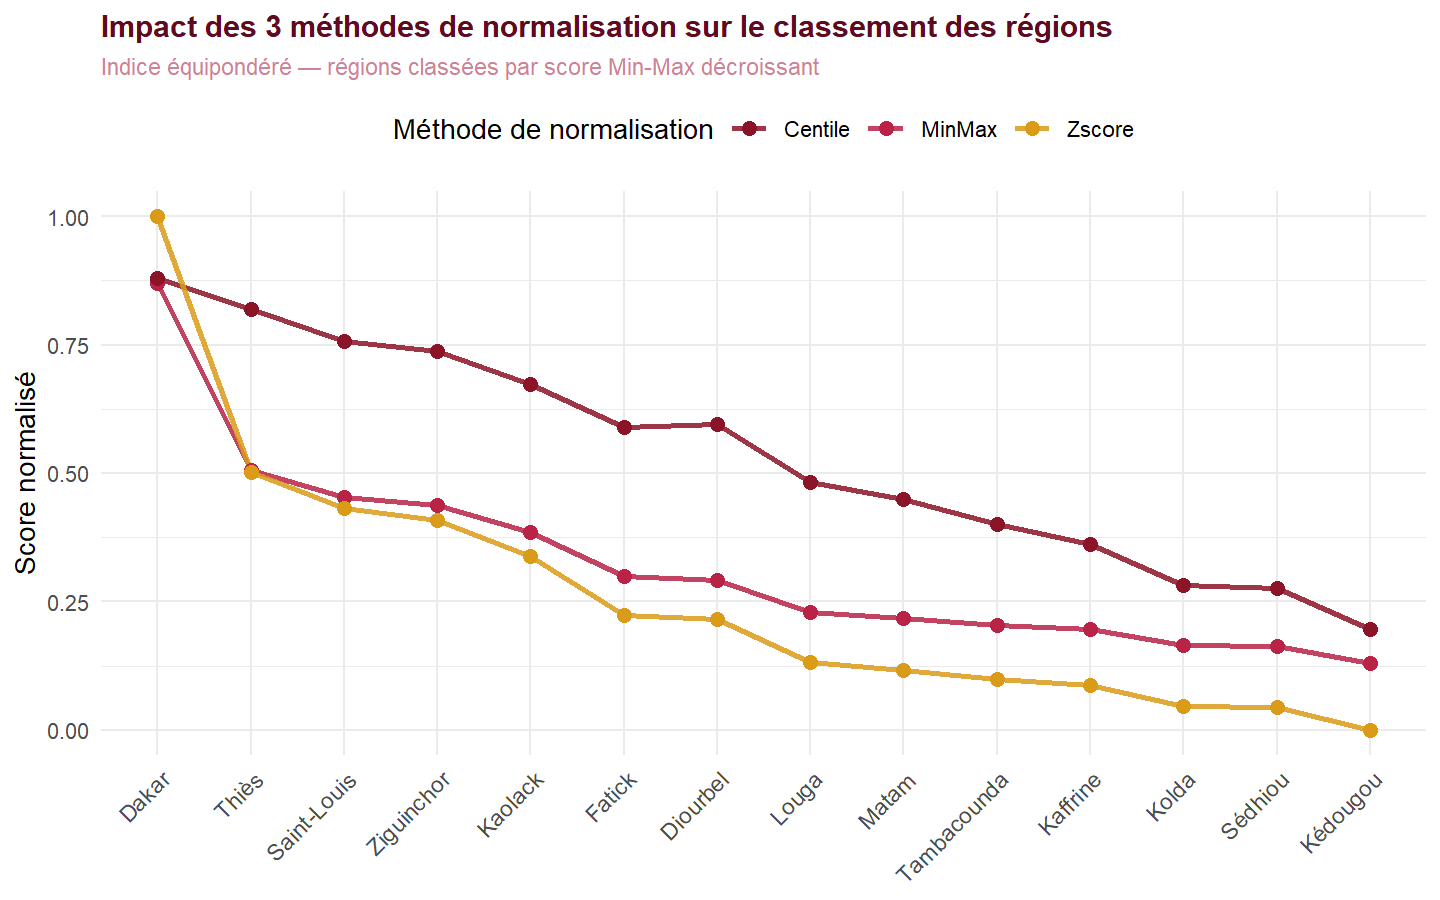
\includegraphics[width=0.9\linewidth]{../figures/rapport-norm-impact-1} 

}

\caption{Impact comparé des trois méthodes de normalisation sur l'indice équipondéré des 14 régions. Les lignes quasi-superposées indiquent une robustesse forte.}\label{fig:norm-impact}
\end{figure}

\textbf{Interprétation :} Les trois courbes sont remarquablement
proches, voire superposées. Cela signifie que le \textbf{choix de la
méthode de normalisation influence très peu le classement final des
régions}. Le signal socioéconomique (gradient Nord-Ouest/Sud-Est) est
suffisamment fort pour primer sur les différences techniques entre
méthodes.

\textbf{Décision méthodologique :} La normalisation \textbf{Min-Max} est
retenue pour la construction de l'indice car elle produit des scores
directement interprétables dans l'intervalle {[}0, 1{]} et facilite la
communication des résultats aux décideurs non statisticiens. La
normalisation Z-score est utilisée comme entrée de l'ACP (recommandation
statistique standard).

\newpage

\section{Étape 3 --- Analyse en Composantes Principales
(ACP)}\label{uxe9tape-3-analyse-en-composantes-principales-acp}

\subsection{Définition et objectifs}\label{duxe9finition-et-objectifs}

\subsubsection{Qu'est-ce que l'ACP ?}\label{quest-ce-que-lacp}

L'\textbf{Analyse en Composantes Principales} (ACP) est une méthode de
statistique multivariée qui transforme un ensemble de variables
corrélées en un ensemble de variables non corrélées appelées
\textbf{composantes principales} ou \textbf{axes factoriels}. Chaque axe
est une combinaison linéaire des variables originales, construite pour
capturer le maximum de variabilité des données.

\textbf{Analogie pédagogique :} Si l'on compare une région à un objet
photographié sous 23 angles différents (23 indicateurs), l'ACP identifie
les 2-3 angles qui donnent le plus d'information sur la forme réelle de
l'objet. On passe de 23 dimensions à quelques dimensions synthétiques
sans perdre l'essentiel de l'information.

\subsubsection{Rôle de l'ACP dans ce
projet}\label{ruxf4le-de-lacp-dans-ce-projet}

L'ACP poursuit ici trois objectifs :

\begin{enumerate}
\def\labelenumi{\arabic{enumi}.}
\tightlist
\item
  \textbf{Réduire la dimensionnalité} : passer de 23 indicateurs à
  quelques axes synthétiques
\item
  \textbf{Identifier les structures latentes} : révéler quelles
  dimensions du développement sont les plus importantes et comment les
  régions se positionnent
\item
  \textbf{Fournir des poids objectifs} : la variance expliquée par
  chaque axe sert à pondérer l'indice de façon statistiquement motivée
\end{enumerate}

\subsection{Paramétrage et résultats de
l'ACP}\label{paramuxe9trage-et-ruxe9sultats-de-lacp}

\begin{Shaded}
\begin{Highlighting}[]
\CommentTok{\# {-}{-} ACP sur les données z{-}score {-}{-}{-}{-}{-}{-}{-}{-}{-}{-}{-}{-}{-}{-}{-}{-}{-}{-}{-}{-}{-}{-}{-}{-}{-}{-}{-}{-}{-}{-}{-}}
\CommentTok{\# On utilise les données Z{-}score (et non Min{-}Max) pour l\textquotesingle{}ACP car :}
\CommentTok{\# 1. L\textquotesingle{}ACP est basée sur la covariance/corrélation entre variables}
\CommentTok{\# 2. Les données Z{-}score sont déjà centrées et réduites}
\CommentTok{\# 3. scale.unit=FALSE : évite une double standardisation}
\CommentTok{\#    (les données sont déjà à variance 1 grâce au Z{-}score)}

\NormalTok{acp    }\OtherTok{\textless{}{-}} \FunctionTok{PCA}\NormalTok{(data\_zs, }\AttributeTok{graph=}\ConstantTok{FALSE}\NormalTok{, }\AttributeTok{scale.unit=}\ConstantTok{FALSE}\NormalTok{)}
\NormalTok{ev     }\OtherTok{\textless{}{-}}\NormalTok{ acp}\SpecialCharTok{$}\NormalTok{eig   }\CommentTok{\# Tableau : valeurs propres, \% variance, \% variance cumulée}
\NormalTok{n\_axes }\OtherTok{\textless{}{-}} \FunctionTok{sum}\NormalTok{(ev[,}\DecValTok{1}\NormalTok{] }\SpecialCharTok{\textgreater{}=} \DecValTok{1}\NormalTok{)  }\CommentTok{\# Critère de Kaiser : garder les axes avec valeur propre \textgreater{}= 1}

\FunctionTok{cat}\NormalTok{(}\StringTok{"=== RÉSULTATS DE L\textquotesingle{}ACP ===}\SpecialCharTok{\textbackslash{}n}\StringTok{"}\NormalTok{)}
\end{Highlighting}
\end{Shaded}

\begin{verbatim}
## === RÉSULTATS DE L'ACP ===
\end{verbatim}

\begin{Shaded}
\begin{Highlighting}[]
\FunctionTok{cat}\NormalTok{(}\FunctionTok{sprintf}\NormalTok{(}\StringTok{"Nombre d\textquotesingle{}axes retenus (critere Kaiser : valeur propre \textgreater{}= 1) : \%d}\SpecialCharTok{\textbackslash{}n}\StringTok{"}\NormalTok{, n\_axes))}
\end{Highlighting}
\end{Shaded}

\begin{verbatim}
## Nombre d'axes retenus (critere Kaiser : valeur propre >= 1) : 2
\end{verbatim}

\begin{Shaded}
\begin{Highlighting}[]
\FunctionTok{cat}\NormalTok{(}\FunctionTok{sprintf}\NormalTok{(}\StringTok{"Variance expliquée par ces \%d axes : \%.1f\%\%}\SpecialCharTok{\textbackslash{}n}\StringTok{"}\NormalTok{, n\_axes, ev[n\_axes, }\DecValTok{3}\NormalTok{]))}
\end{Highlighting}
\end{Shaded}

\begin{verbatim}
## Variance expliquée par ces 2 axes : 98.5%
\end{verbatim}

\begin{Shaded}
\begin{Highlighting}[]
\FunctionTok{cat}\NormalTok{(}\StringTok{"}\SpecialCharTok{\textbackslash{}n}\StringTok{Tableau complet des 5 premiers axes :}\SpecialCharTok{\textbackslash{}n}\StringTok{"}\NormalTok{)}
\end{Highlighting}
\end{Shaded}

\begin{verbatim}
## 
## Tableau complet des 5 premiers axes :
\end{verbatim}

\begin{Shaded}
\begin{Highlighting}[]
\NormalTok{tab\_ev }\OtherTok{\textless{}{-}} \FunctionTok{data.frame}\NormalTok{(}
  \AttributeTok{Axe        =} \FunctionTok{paste}\NormalTok{(}\StringTok{"Dim."}\NormalTok{, }\DecValTok{1}\SpecialCharTok{:}\FunctionTok{min}\NormalTok{(}\DecValTok{5}\NormalTok{, }\FunctionTok{nrow}\NormalTok{(ev))),}
  \AttributeTok{Val\_propre =} \FunctionTok{round}\NormalTok{(ev[}\DecValTok{1}\SpecialCharTok{:}\FunctionTok{min}\NormalTok{(}\DecValTok{5}\NormalTok{,}\FunctionTok{nrow}\NormalTok{(ev)), }\DecValTok{1}\NormalTok{], }\DecValTok{3}\NormalTok{),}
  \AttributeTok{Variance   =} \FunctionTok{paste0}\NormalTok{(}\FunctionTok{round}\NormalTok{(ev[}\DecValTok{1}\SpecialCharTok{:}\FunctionTok{min}\NormalTok{(}\DecValTok{5}\NormalTok{,}\FunctionTok{nrow}\NormalTok{(ev)), }\DecValTok{2}\NormalTok{], }\DecValTok{1}\NormalTok{), }\StringTok{"\%"}\NormalTok{),}
  \AttributeTok{Cumulee    =} \FunctionTok{paste0}\NormalTok{(}\FunctionTok{round}\NormalTok{(ev[}\DecValTok{1}\SpecialCharTok{:}\FunctionTok{min}\NormalTok{(}\DecValTok{5}\NormalTok{,}\FunctionTok{nrow}\NormalTok{(ev)), }\DecValTok{3}\NormalTok{], }\DecValTok{1}\NormalTok{), }\StringTok{"\%"}\NormalTok{)}
\NormalTok{)}
\FunctionTok{print}\NormalTok{(tab\_ev)}
\end{Highlighting}
\end{Shaded}

\begin{verbatim}
##           Axe Val_propre Variance Cumulee
## comp 1 Dim. 1     20.029    93.8%   93.8%
## comp 2 Dim. 2      1.014     4.7%   98.5%
## comp 3 Dim. 3      0.187     0.9%   99.4%
## comp 4 Dim. 4      0.057     0.3%   99.7%
## comp 5 Dim. 5      0.026     0.1%   99.8%
\end{verbatim}

\textbf{Interprétation des valeurs propres :} La valeur propre mesure la
quantité d'information capturée par chaque axe. Une valeur propre de 15
signifie que cet axe résume autant d'information que 15 indicateurs
originaux pris ensemble. Le \textbf{critère de Kaiser} (valeur propre
\(\geq\) 1) garantit que chaque axe retenu apporte au moins autant
d'information qu'un indicateur original.

\subsection{Éboulis des valeurs
propres}\label{uxe9boulis-des-valeurs-propres}

\begin{Shaded}
\begin{Highlighting}[]
\CommentTok{\# L\textquotesingle{}éboulis ("screeplot") représente graphiquement les valeurs propres}
\CommentTok{\# par ordre décroissant. Le "coude" de la courbe indique combien d\textquotesingle{}axes}
\CommentTok{\# on devrait retenir selon le critère visuel de Cattell.}

\FunctionTok{fviz\_eig}\NormalTok{(acp,}
  \AttributeTok{addlabels =} \ConstantTok{TRUE}\NormalTok{,       }\CommentTok{\# Afficher les \% sur chaque barre}
  \AttributeTok{ylim      =} \FunctionTok{c}\NormalTok{(}\DecValTok{0}\NormalTok{, }\DecValTok{82}\NormalTok{),}
  \AttributeTok{barfill   =}\NormalTok{ CV,         }\CommentTok{\# Couleur vert forêt pour les barres}
  \AttributeTok{barcolor  =}\NormalTok{ CV,}
  \AttributeTok{linecolor =}\NormalTok{ C3,         }\CommentTok{\# Ligne en or pour la courbe cumulative}
  \AttributeTok{ggtheme   =} \FunctionTok{theme\_minimal}\NormalTok{(}\AttributeTok{base\_size=}\DecValTok{11}\NormalTok{)) }\SpecialCharTok{+}
  \FunctionTok{labs}\NormalTok{(}
    \AttributeTok{title    =} \StringTok{"Éboulis des valeurs propres de l\textquotesingle{}ACP"}\NormalTok{,}
    \AttributeTok{subtitle =} \FunctionTok{paste0}\NormalTok{(n\_axes, }\StringTok{" axe(s) retenu(s) {-} critere de Kaiser (valeur propre \textgreater{}= 1) {-} "}\NormalTok{,}
                      \FunctionTok{round}\NormalTok{(ev[n\_axes, }\DecValTok{3}\NormalTok{], }\DecValTok{1}\NormalTok{), }\StringTok{"\% de variance totale expliquee"}\NormalTok{),}
    \AttributeTok{x =} \StringTok{"Composante principale (Axe)"}\NormalTok{,}
    \AttributeTok{y =} \StringTok{"Variance expliquée (\%)"}
\NormalTok{  ) }\SpecialCharTok{+}
  \FunctionTok{theme}\NormalTok{(}
    \AttributeTok{plot.title    =} \FunctionTok{element\_text}\NormalTok{(}\AttributeTok{face=}\StringTok{"bold"}\NormalTok{, }\AttributeTok{color=}\NormalTok{C4, }\AttributeTok{size=}\DecValTok{12}\NormalTok{),}
    \AttributeTok{plot.subtitle =} \FunctionTok{element\_text}\NormalTok{(}\AttributeTok{color=}\NormalTok{C5, }\AttributeTok{size=}\FloatTok{9.5}\NormalTok{),}
    \AttributeTok{axis.title    =} \FunctionTok{element\_text}\NormalTok{(}\AttributeTok{color=}\NormalTok{C4, }\AttributeTok{size=}\DecValTok{10}\NormalTok{)}
\NormalTok{  )}
\end{Highlighting}
\end{Shaded}

\begin{figure}

{\centering 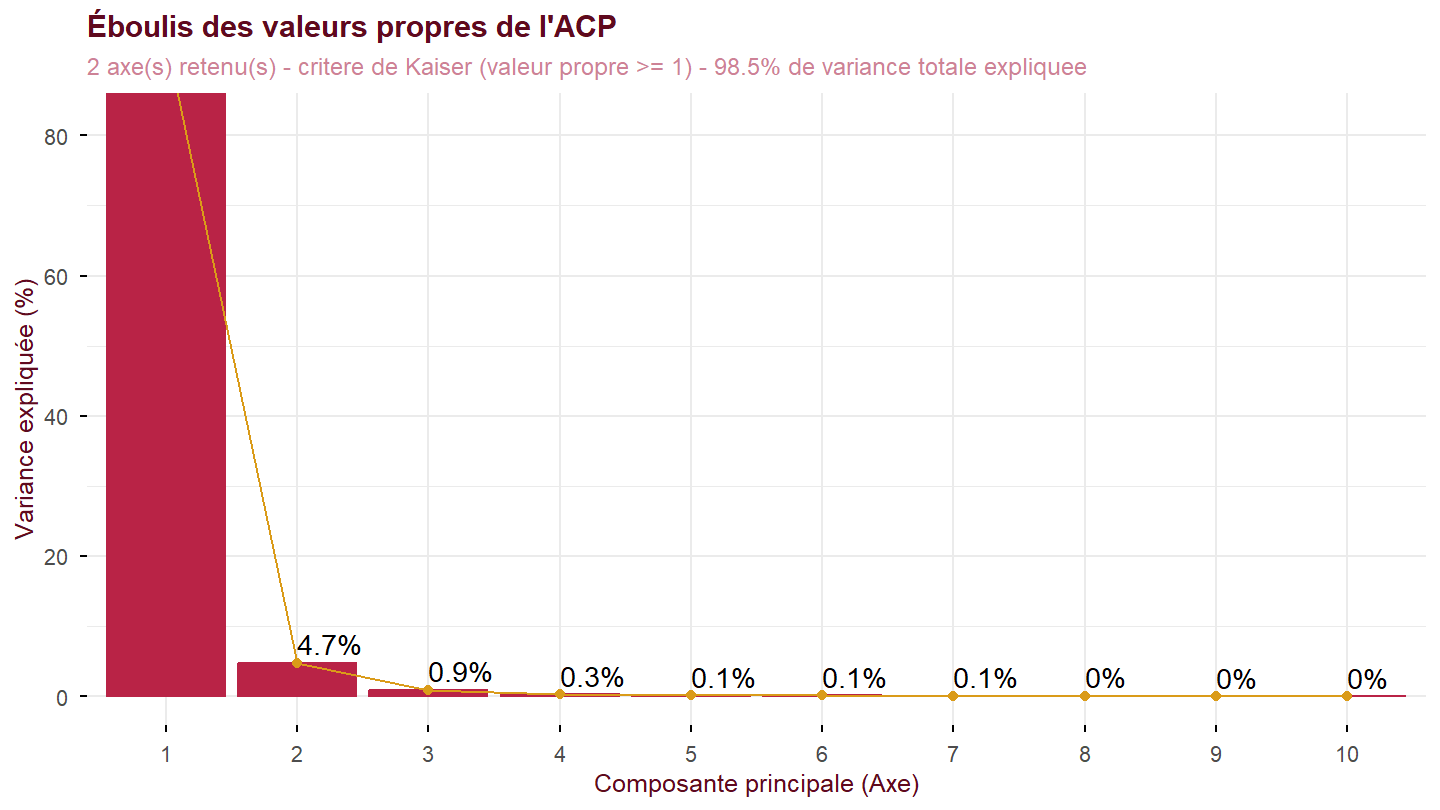
\includegraphics[width=0.9\linewidth]{../figures/rapport-scree-1} 

}

\caption{Éboulis des valeurs propres (Screeplot). Le coude prononcé après l'Axe 1 illustre sa domination dans la structure des données.}\label{fig:scree}
\end{figure}

\textbf{Interprétation :} L'Axe 1 capture à lui seul la grande majorité
de la variance totale. Ce résultat révèle que le développement au
Sénégal est fortement \textbf{unidimensionnel} : les régions se classent
quasi-linéairement sur un seul gradient, du plus développé au moins
développé. C'est cohérent avec la réalité sénégalaise où toutes les
dimensions (éducation, santé, revenus, infrastructure) sont fortement
corrélées et suivent le même gradient géographique Nord-Ouest/Sud-Est.

\subsection{Biplot ACP --- Visualisation des régions et des
indicateurs}\label{biplot-acp-visualisation-des-ruxe9gions-et-des-indicateurs}

\begin{Shaded}
\begin{Highlighting}[]
\CommentTok{\# Le biplot combine les deux types d\textquotesingle{}informations en un seul graphique :}
\CommentTok{\# {-} Les POINTS (individus / régions) : leur position révèle leur niveau global}
\CommentTok{\#   sur chaque axe. Une région à droite sur l\textquotesingle{}Axe 1 = bien développée.}
\CommentTok{\# {-} Les FLÈCHES (variables / indicateurs) : leur direction et longueur révèlent}
\CommentTok{\#   leur contribution à chaque axe. Une longue flèche vers la droite sur l\textquotesingle{}Axe 1}
\CommentTok{\#   = cet indicateur discrimine fortement les régions développées des autres.}
\CommentTok{\# {-} L\textquotesingle{}ANGLE entre deux flèches indique leur corrélation (0° = corrélés positivement,}
\CommentTok{\#   180° = corrélés négativement, 90° = non corrélés).}

\FunctionTok{fviz\_pca\_biplot}\NormalTok{(acp,}
  \AttributeTok{repel   =} \ConstantTok{TRUE}\NormalTok{,         }\CommentTok{\# Éviter que les labels se chevauchent}
  \AttributeTok{col.var =}\NormalTok{ C3,           }\CommentTok{\# Couleur or pour les indicateurs (flèches)}
  \AttributeTok{col.ind =}\NormalTok{ CV,           }\CommentTok{\# Couleur verte pour les régions (points)}
  \AttributeTok{label   =} \StringTok{"all"}\NormalTok{,        }\CommentTok{\# Afficher tous les labels}
  \AttributeTok{ggtheme =} \FunctionTok{theme\_minimal}\NormalTok{(}\AttributeTok{base\_size=}\DecValTok{9}\NormalTok{),}
  \AttributeTok{title   =} \StringTok{"Biplot ACP {-} Regions (points) et indicateurs (fleches)"}\NormalTok{) }\SpecialCharTok{+}
  \FunctionTok{theme}\NormalTok{(}
    \AttributeTok{plot.title =} \FunctionTok{element\_text}\NormalTok{(}\AttributeTok{face=}\StringTok{"bold"}\NormalTok{, }\AttributeTok{color=}\NormalTok{C4, }\AttributeTok{size=}\DecValTok{11}\NormalTok{),}
    \AttributeTok{axis.title =} \FunctionTok{element\_text}\NormalTok{(}\AttributeTok{color=}\NormalTok{C4, }\AttributeTok{size=}\FloatTok{9.5}\NormalTok{)}
\NormalTok{  )}
\end{Highlighting}
\end{Shaded}

\begin{figure}

{\centering 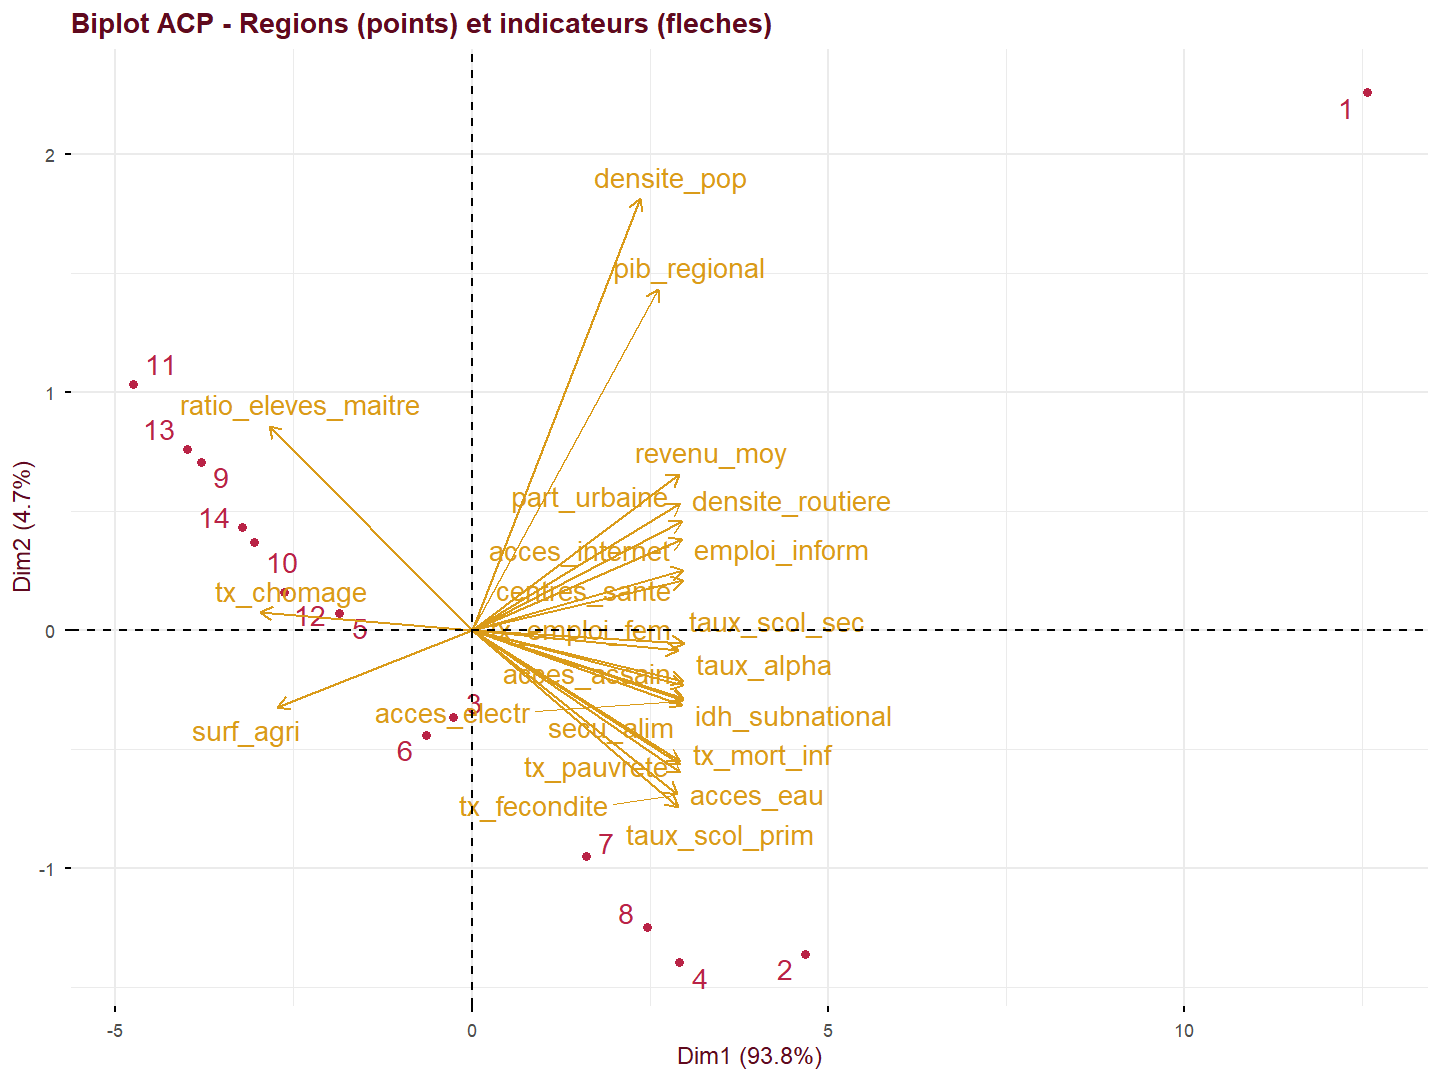
\includegraphics[width=0.9\linewidth]{../figures/rapport-biplot-1} 

}

\caption{Biplot ACP : les points (régions) et les flèches (indicateurs) représentés dans l'espace des deux premiers axes. Dakar est clairement isolé à droite, tandis que Kédougou, Sédhiou et Kolda sont regroupés à gauche.}\label{fig:biplot}
\end{figure}

\textbf{Interprétation du biplot :}

\begin{itemize}
\tightlist
\item
  \textbf{Dakar} se positionne à l'extrême droite de l'Axe 1, très loin
  des autres régions : c'est clairement un \textbf{outlier positif} sur
  toutes les dimensions.
\item
  \textbf{Kédougou, Sédhiou, Kolda} sont regroupés à l'extrême gauche :
  leurs profils socioéconomiques défavorables sont similaires entre eux,
  traduisant un \textbf{enclavement structurel} commun.
\item
  \textbf{L'Axe 2} oppose les régions à forte densité et urbanisation
  (Dakar) aux régions essentiellement rurales et agricoles. Les
  indicateurs d'infrastructure et d'internet pointent vers le
  haut-droite, illustrant leur concentration dans les régions les plus
  urbanisées.
\item
  Les flèches d'indicateurs de la même dimension (ex. taux
  d'alphabétisation + scolarisation primaire + scolarisation secondaire)
  pointent dans la même direction, confirmant leur cohérence thématique.
\end{itemize}

\subsection{Dimensions latentes
identifiées}\label{dimensions-latentes-identifiuxe9es}

\begingroup\fontsize{9}{11}\selectfont

\begin{longtable}[t]{llrl>{\raggedright\arraybackslash}p{9cm}l}
\caption{\label{tab:dim-tab}Résumé et interprétation des 3 premiers axes de l'ACP}\\
\toprule
 & Axe & Val. propre & Variance & Cumulée & Signification thématique\\
\midrule
\cellcolor{gray!10}{comp 1} & \cellcolor{gray!10}{Axe 1} & \cellcolor{gray!10}{20.03} & \cellcolor{gray!10}{93.8\%} & \cellcolor{gray!10}{93.8\%} & \cellcolor{gray!10}{Développement humain global : oppose les régions bien dotées en éducation, santé, revenus et services (Dakar, Thiès) aux régions défavorisées (Kédougou, Sédhiou, Kolda)}\\
comp 2 & Axe 2 & 1.01 & 4.7\% & 98.5\% & Infrastructure et connectivité : différencie les régions selon leur accès aux routes, internet et électricité, indépendamment du niveau général de développement\\
\cellcolor{gray!10}{comp 3} & \cellcolor{gray!10}{Axe 3} & \cellcolor{gray!10}{0.19} & \cellcolor{gray!10}{0.9\%} & \cellcolor{gray!10}{99.4\%} & \cellcolor{gray!10}{Structure démographique : oppose les régions à forte fécondité et ruralité aux régions plus urbanisées et avec un emploi féminin développé}\\
\bottomrule
\end{longtable}
\endgroup{}

\newpage

\section{Étape 4 --- Construction des indices
composites}\label{uxe9tape-4-construction-des-indices-composites}

\subsection{Système 1 ---
Équipondération}\label{systuxe8me-1-uxe9quiponduxe9ration}

\begin{Shaded}
\begin{Highlighting}[]
\CommentTok{\# {-}{-} Indice 1 : Équipondération {-}{-}{-}{-}{-}{-}{-}{-}{-}{-}{-}{-}{-}{-}{-}{-}{-}{-}{-}{-}{-}{-}{-}{-}{-}{-}{-}{-}{-}{-}{-}{-}}
\CommentTok{\# Principe : chaque indicateur reçoit le même poids (1/23 \textasciitilde{} 4,35\%)}
\CommentTok{\# L\textquotesingle{}indice est simplement la moyenne des 23 indicateurs normalisés}
\CommentTok{\# Formule : I\_equi = (1/23) x S x*\_i pour i = 1 à 23}

\NormalTok{indice\_equi }\OtherTok{\textless{}{-}} \FunctionTok{rowMeans}\NormalTok{(data\_mm)}

\FunctionTok{cat}\NormalTok{(}\StringTok{"=== INDICE ÉQUIPONDÉRÉ ===}\SpecialCharTok{\textbackslash{}n}\StringTok{"}\NormalTok{)}
\end{Highlighting}
\end{Shaded}

\begin{verbatim}
## === INDICE ÉQUIPONDÉRÉ ===
\end{verbatim}

\begin{Shaded}
\begin{Highlighting}[]
\FunctionTok{cat}\NormalTok{(}\FunctionTok{sprintf}\NormalTok{(}\StringTok{"Plage de l\textquotesingle{}indice : [\%.3f ; \%.3f]}\SpecialCharTok{\textbackslash{}n}\StringTok{"}\NormalTok{, }\FunctionTok{min}\NormalTok{(indice\_equi), }\FunctionTok{max}\NormalTok{(indice\_equi)))}
\end{Highlighting}
\end{Shaded}

\begin{verbatim}
## Plage de l'indice : [0.130 ; 0.870]
\end{verbatim}

\begin{Shaded}
\begin{Highlighting}[]
\FunctionTok{cat}\NormalTok{(}\FunctionTok{sprintf}\NormalTok{(}\StringTok{"Moyenne des 14 régions : \%.3f}\SpecialCharTok{\textbackslash{}n}\StringTok{"}\NormalTok{, }\FunctionTok{mean}\NormalTok{(indice\_equi)))}
\end{Highlighting}
\end{Shaded}

\begin{verbatim}
## Moyenne des 14 régions : 0.325
\end{verbatim}

\begin{Shaded}
\begin{Highlighting}[]
\FunctionTok{cat}\NormalTok{(}\StringTok{"}\SpecialCharTok{\textbackslash{}n}\StringTok{Résultats par région :}\SpecialCharTok{\textbackslash{}n}\StringTok{"}\NormalTok{)}
\end{Highlighting}
\end{Shaded}

\begin{verbatim}
## 
## Résultats par région :
\end{verbatim}

\begin{Shaded}
\begin{Highlighting}[]
\NormalTok{tab\_eq }\OtherTok{\textless{}{-}} \FunctionTok{data.frame}\NormalTok{(}
\NormalTok{  Région }\OtherTok{=}\NormalTok{ regions,}
  \AttributeTok{Score  =} \FunctionTok{round}\NormalTok{(indice\_equi, }\DecValTok{3}\NormalTok{),}
  \AttributeTok{Rang   =} \FunctionTok{rank}\NormalTok{(}\SpecialCharTok{{-}}\NormalTok{indice\_equi)}
\NormalTok{) }\SpecialCharTok{\%\textgreater{}\%} \FunctionTok{arrange}\NormalTok{(Rang)}
\FunctionTok{print}\NormalTok{(tab\_eq)}
\end{Highlighting}
\end{Shaded}

\begin{verbatim}
##         Région Score Rang
## 1        Dakar 0.870    1
## 2        Thiès 0.506    2
## 3  Saint-Louis 0.454    3
## 4   Ziguinchor 0.437    4
## 5      Kaolack 0.385    5
## 6       Fatick 0.299    6
## 7     Diourbel 0.291    7
## 8        Louga 0.229    8
## 9        Matam 0.218    9
## 10 Tambacounda 0.204   10
## 11    Kaffrine 0.196   11
## 12       Kolda 0.165   12
## 13     Sédhiou 0.163   13
## 14    Kédougou 0.130   14
\end{verbatim}

\textbf{Avantages et limites :} L'équipondération est simple et
transparente. Cependant, elle constitue un \textbf{choix politique
implicite} : elle suppose que la densité routière est aussi importante
que la mortalité infantile dans la mesure du développement. Ce n'est pas
une neutralité --- c'est une prise de position qui devrait être
explicitée.

\subsection{Système 2 --- Pondération par
l'ACP}\label{systuxe8me-2-ponduxe9ration-par-lacp}

\begin{Shaded}
\begin{Highlighting}[]
\CommentTok{\# {-}{-} Indice 2 : Pondération ACP {-}{-}{-}{-}{-}{-}{-}{-}{-}{-}{-}{-}{-}{-}{-}{-}{-}{-}{-}{-}{-}{-}{-}{-}{-}{-}{-}{-}{-}{-}{-}{-}}
\CommentTok{\# Principe : les axes ACP qui expliquent le plus de variance}
\CommentTok{\# reçoivent le plus de poids. C\textquotesingle{}est une pondération "objective"}
\CommentTok{\# car elle émerge des données elles{-}mêmes.}

\CommentTok{\# Calcul des poids : poids de l\textquotesingle{}axe k = variance\_k / variance\_totale\_retenue}
\NormalTok{poids\_acp\_val }\OtherTok{\textless{}{-}}\NormalTok{ ev[}\DecValTok{1}\SpecialCharTok{:}\NormalTok{n\_axes, }\DecValTok{2}\NormalTok{] }\SpecialCharTok{/} \FunctionTok{sum}\NormalTok{(ev[}\DecValTok{1}\SpecialCharTok{:}\NormalTok{n\_axes, }\DecValTok{2}\NormalTok{])}

\FunctionTok{cat}\NormalTok{(}\StringTok{"=== POIDS ACP PAR AXE ===}\SpecialCharTok{\textbackslash{}n}\StringTok{"}\NormalTok{)}
\end{Highlighting}
\end{Shaded}

\begin{verbatim}
## === POIDS ACP PAR AXE ===
\end{verbatim}

\begin{Shaded}
\begin{Highlighting}[]
\ControlFlowTok{for}\NormalTok{(i }\ControlFlowTok{in} \DecValTok{1}\SpecialCharTok{:}\NormalTok{n\_axes) \{}
  \FunctionTok{cat}\NormalTok{(}\FunctionTok{sprintf}\NormalTok{(}\StringTok{"  Axe \%d : poids = \%.1f\%\% (valeur propre = \%.2f)}\SpecialCharTok{\textbackslash{}n}\StringTok{"}\NormalTok{,}
\NormalTok{              i, poids\_acp\_val[i]}\SpecialCharTok{*}\DecValTok{100}\NormalTok{, ev[i,}\DecValTok{1}\NormalTok{]))}
\NormalTok{\}}
\end{Highlighting}
\end{Shaded}

\begin{verbatim}
##   Axe 1 : poids = 95.2% (valeur propre = 20.03)
##   Axe 2 : poids = 4.8% (valeur propre = 1.01)
\end{verbatim}

\begin{Shaded}
\begin{Highlighting}[]
\CommentTok{\# Calcul de l\textquotesingle{}indice : combinaison linéaire des coordonnées ACP pondérées}
\NormalTok{coord\_axes   }\OtherTok{\textless{}{-}} \FunctionTok{as.data.frame}\NormalTok{(acp}\SpecialCharTok{$}\NormalTok{ind}\SpecialCharTok{$}\NormalTok{coord[, }\DecValTok{1}\SpecialCharTok{:}\NormalTok{n\_axes])}
\NormalTok{coord\_mm\_acp }\OtherTok{\textless{}{-}} \FunctionTok{as.data.frame}\NormalTok{(}\FunctionTok{lapply}\NormalTok{(coord\_axes, minmax))  }\CommentTok{\# Normaliser les coordonnées}
\NormalTok{indice\_acp   }\OtherTok{\textless{}{-}} \FunctionTok{as.numeric}\NormalTok{(}\FunctionTok{as.matrix}\NormalTok{(coord\_mm\_acp) }\SpecialCharTok{\%*\%}\NormalTok{ poids\_acp\_val)}

\FunctionTok{cat}\NormalTok{(}\FunctionTok{sprintf}\NormalTok{(}\StringTok{"}\SpecialCharTok{\textbackslash{}n}\StringTok{Plage de l\textquotesingle{}indice ACP : [\%.3f ; \%.3f]}\SpecialCharTok{\textbackslash{}n}\StringTok{"}\NormalTok{,}
            \FunctionTok{min}\NormalTok{(indice\_acp), }\FunctionTok{max}\NormalTok{(indice\_acp)))}
\end{Highlighting}
\end{Shaded}

\begin{verbatim}
## 
## Plage de l'indice ACP : [0.032 ; 1.000]
\end{verbatim}

\subsection{Système 3 --- Pondération AHP par
dimension}\label{systuxe8me-3-ponduxe9ration-ahp-par-dimension}

\begin{Shaded}
\begin{Highlighting}[]
\CommentTok{\# {-}{-} Indice 3 : Pondération AHP {-}{-}{-}{-}{-}{-}{-}{-}{-}{-}{-}{-}{-}{-}{-}{-}{-}{-}{-}{-}{-}{-}{-}{-}{-}{-}{-}{-}{-}{-}{-}{-}}
\CommentTok{\# L\textquotesingle{}AHP (Analytic Hierarchy Process) procède en deux niveaux :}
\CommentTok{\# NIVEAU 1 : on regroupe les indicateurs par dimension thématique}
\CommentTok{\#            et on calcule un score moyen par dimension}
\CommentTok{\# NIVEAU 2 : on combine les scores de dimension avec des poids}
\CommentTok{\#            définis par jugement d\textquotesingle{}expert (comparaisons par paires)}

\CommentTok{\# Définition des indicateurs par dimension thématique}
\NormalTok{dim\_edu }\OtherTok{\textless{}{-}} \FunctionTok{c}\NormalTok{(}\StringTok{"taux\_alpha"}\NormalTok{,}\StringTok{"taux\_scol\_prim"}\NormalTok{,}\StringTok{"taux\_scol\_sec"}\NormalTok{,}\StringTok{"ratio\_eleves\_maitre"}\NormalTok{)}
\NormalTok{dim\_san }\OtherTok{\textless{}{-}} \FunctionTok{c}\NormalTok{(}\StringTok{"tx\_mort\_inf"}\NormalTok{,}\StringTok{"acces\_eau"}\NormalTok{,}\StringTok{"acces\_assain"}\NormalTok{,}\StringTok{"centres\_sante"}\NormalTok{)}
\NormalTok{dim\_eco }\OtherTok{\textless{}{-}} \FunctionTok{c}\NormalTok{(}\StringTok{"tx\_pauvrete"}\NormalTok{,}\StringTok{"revenu\_moy"}\NormalTok{,}\StringTok{"tx\_chomage"}\NormalTok{,}\StringTok{"emploi\_inform"}\NormalTok{,}\StringTok{"pib\_regional"}\NormalTok{)}
\NormalTok{dim\_inf }\OtherTok{\textless{}{-}} \FunctionTok{c}\NormalTok{(}\StringTok{"acces\_electr"}\NormalTok{,}\StringTok{"densite\_routiere"}\NormalTok{,}\StringTok{"acces\_internet"}\NormalTok{,}\StringTok{"idh\_subnational"}\NormalTok{)}
\NormalTok{dim\_dem }\OtherTok{\textless{}{-}} \FunctionTok{c}\NormalTok{(}\StringTok{"tx\_fecondite"}\NormalTok{,}\StringTok{"densite\_pop"}\NormalTok{,}\StringTok{"part\_urbaine"}\NormalTok{,}\StringTok{"tx\_emploi\_fem"}\NormalTok{,}\StringTok{"surf\_agri"}\NormalTok{,}\StringTok{"secu\_alim"}\NormalTok{)}

\CommentTok{\# Calcul du score moyen de chaque région dans chaque dimension}
\NormalTok{sc\_edu }\OtherTok{\textless{}{-}} \FunctionTok{rowMeans}\NormalTok{(data\_mm[, dim\_edu])  }\CommentTok{\# Score Éducation}
\NormalTok{sc\_san }\OtherTok{\textless{}{-}} \FunctionTok{rowMeans}\NormalTok{(data\_mm[, dim\_san])  }\CommentTok{\# Score Santé}
\NormalTok{sc\_eco }\OtherTok{\textless{}{-}} \FunctionTok{rowMeans}\NormalTok{(data\_mm[, dim\_eco])  }\CommentTok{\# Score Économie}
\NormalTok{sc\_inf }\OtherTok{\textless{}{-}} \FunctionTok{rowMeans}\NormalTok{(data\_mm[, dim\_inf])  }\CommentTok{\# Score Infrastructure}
\NormalTok{sc\_dem }\OtherTok{\textless{}{-}} \FunctionTok{rowMeans}\NormalTok{(data\_mm[, dim\_dem])  }\CommentTok{\# Score Démographie}

\CommentTok{\# Poids AHP par dimension (issus d\textquotesingle{}une comparaison par paires d\textquotesingle{}expert) :}
\CommentTok{\# {-} Éducation   : 25\% (levier de développement à long terme)}
\CommentTok{\# {-} Économie    : 25\% (capacité à générer des revenus et emplois formels)}
\CommentTok{\# {-} Santé       : 20\% (bien{-}être physique et survie)}
\CommentTok{\# {-} Infrastructure : 20\% (connectivité et accès aux services de base)}
\CommentTok{\# {-} Démographie : 10\% (structure de population, moins directement actionnable)}
\CommentTok{\# VÉRIFICATION : 25 + 25 + 20 + 20 + 10 = 100\% OK}
\NormalTok{indice\_ahp }\OtherTok{\textless{}{-}} \FloatTok{0.25}\SpecialCharTok{*}\NormalTok{sc\_edu }\SpecialCharTok{+} \FloatTok{0.25}\SpecialCharTok{*}\NormalTok{sc\_eco }\SpecialCharTok{+} \FloatTok{0.20}\SpecialCharTok{*}\NormalTok{sc\_san }\SpecialCharTok{+} \FloatTok{0.20}\SpecialCharTok{*}\NormalTok{sc\_inf }\SpecialCharTok{+} \FloatTok{0.10}\SpecialCharTok{*}\NormalTok{sc\_dem}

\FunctionTok{cat}\NormalTok{(}\StringTok{"=== POIDS AHP PAR DIMENSION ===}\SpecialCharTok{\textbackslash{}n}\StringTok{"}\NormalTok{)}
\end{Highlighting}
\end{Shaded}

\begin{verbatim}
## === POIDS AHP PAR DIMENSION ===
\end{verbatim}

\begin{Shaded}
\begin{Highlighting}[]
\FunctionTok{cat}\NormalTok{(}\StringTok{"  Éducation      : 25\%}\SpecialCharTok{\textbackslash{}n}\StringTok{"}\NormalTok{)}
\end{Highlighting}
\end{Shaded}

\begin{verbatim}
##   Éducation      : 25%
\end{verbatim}

\begin{Shaded}
\begin{Highlighting}[]
\FunctionTok{cat}\NormalTok{(}\StringTok{"  Économie       : 25\%}\SpecialCharTok{\textbackslash{}n}\StringTok{"}\NormalTok{)}
\end{Highlighting}
\end{Shaded}

\begin{verbatim}
##   Économie       : 25%
\end{verbatim}

\begin{Shaded}
\begin{Highlighting}[]
\FunctionTok{cat}\NormalTok{(}\StringTok{"  Santé          : 20\%}\SpecialCharTok{\textbackslash{}n}\StringTok{"}\NormalTok{)}
\end{Highlighting}
\end{Shaded}

\begin{verbatim}
##   Santé          : 20%
\end{verbatim}

\begin{Shaded}
\begin{Highlighting}[]
\FunctionTok{cat}\NormalTok{(}\StringTok{"  Infrastructure : 20\%}\SpecialCharTok{\textbackslash{}n}\StringTok{"}\NormalTok{)}
\end{Highlighting}
\end{Shaded}

\begin{verbatim}
##   Infrastructure : 20%
\end{verbatim}

\begin{Shaded}
\begin{Highlighting}[]
\FunctionTok{cat}\NormalTok{(}\StringTok{"  Démographie    : 10\%}\SpecialCharTok{\textbackslash{}n}\StringTok{"}\NormalTok{)}
\end{Highlighting}
\end{Shaded}

\begin{verbatim}
##   Démographie    : 10%
\end{verbatim}

\begin{Shaded}
\begin{Highlighting}[]
\FunctionTok{cat}\NormalTok{(}\StringTok{"  TOTAL          : 100\%}\SpecialCharTok{\textbackslash{}n\textbackslash{}n}\StringTok{"}\NormalTok{)}
\end{Highlighting}
\end{Shaded}

\begin{verbatim}
##   TOTAL          : 100%
\end{verbatim}

\begin{Shaded}
\begin{Highlighting}[]
\FunctionTok{cat}\NormalTok{(}\FunctionTok{sprintf}\NormalTok{(}\StringTok{"Plage de l\textquotesingle{}indice AHP : [\%.3f ; \%.3f]}\SpecialCharTok{\textbackslash{}n}\StringTok{"}\NormalTok{,}
            \FunctionTok{min}\NormalTok{(indice\_ahp), }\FunctionTok{max}\NormalTok{(indice\_ahp)))}
\end{Highlighting}
\end{Shaded}

\begin{verbatim}
## Plage de l'indice AHP : [0.129 ; 0.871]
\end{verbatim}

\subsection{Profil multidimensionnel des
régions}\label{profil-multidimensionnel-des-ruxe9gions}

\begin{Shaded}
\begin{Highlighting}[]
\CommentTok{\# Ce graphique présente le profil de chaque région dans les 5 dimensions}
\CommentTok{\# Chaque barre représente le score normalisé [0,1] de la région dans une dimension}
\CommentTok{\# Permet d\textquotesingle{}identifier les forces et faiblesses spécifiques de chaque région}

\NormalTok{scores\_df }\OtherTok{\textless{}{-}} \FunctionTok{data.frame}\NormalTok{(}
  \AttributeTok{Region        =}\NormalTok{ regions,}
  \AttributeTok{Education     =}\NormalTok{ sc\_edu,}
  \AttributeTok{Sante         =}\NormalTok{ sc\_san,}
  \AttributeTok{Economie      =}\NormalTok{ sc\_eco,}
  \AttributeTok{Infrastructure=}\NormalTok{ sc\_inf,}
  \AttributeTok{Demographie   =}\NormalTok{ sc\_dem}
\NormalTok{) }\SpecialCharTok{\%\textgreater{}\%}
  \FunctionTok{pivot\_longer}\NormalTok{(}\SpecialCharTok{{-}}\NormalTok{Region, }\AttributeTok{names\_to=}\StringTok{"Dimension"}\NormalTok{, }\AttributeTok{values\_to=}\StringTok{"Score"}\NormalTok{) }\SpecialCharTok{\%\textgreater{}\%}
  \FunctionTok{mutate}\NormalTok{(}\AttributeTok{Region =} \FunctionTok{factor}\NormalTok{(Region,}
                         \AttributeTok{levels=}\NormalTok{regions[}\FunctionTok{order}\NormalTok{(}\FunctionTok{as.numeric}\NormalTok{(indice\_ahp), }\AttributeTok{decreasing=}\ConstantTok{TRUE}\NormalTok{)]))}

\FunctionTok{ggplot}\NormalTok{(scores\_df, }\FunctionTok{aes}\NormalTok{(}\AttributeTok{x=}\NormalTok{Dimension, }\AttributeTok{y=}\NormalTok{Score, }\AttributeTok{fill=}\NormalTok{Dimension)) }\SpecialCharTok{+}
  \FunctionTok{geom\_bar}\NormalTok{(}\AttributeTok{stat=}\StringTok{"identity"}\NormalTok{, }\AttributeTok{width=}\FloatTok{0.75}\NormalTok{) }\SpecialCharTok{+}
  \FunctionTok{facet\_wrap}\NormalTok{(}\SpecialCharTok{\textasciitilde{}}\NormalTok{Region, }\AttributeTok{ncol=}\DecValTok{5}\NormalTok{) }\SpecialCharTok{+}
  \FunctionTok{scale\_fill\_manual}\NormalTok{(}
    \AttributeTok{values=}\FunctionTok{c}\NormalTok{(}\AttributeTok{Education=}\NormalTok{CV, }\AttributeTok{Sante=}\NormalTok{C2, }\AttributeTok{Economie=}\NormalTok{C3, }\AttributeTok{Infrastructure=}\StringTok{"\#8C6914"}\NormalTok{, }\AttributeTok{Demographie=}\NormalTok{C5)}
\NormalTok{  ) }\SpecialCharTok{+}
  \FunctionTok{labs}\NormalTok{(}
    \AttributeTok{title    =} \StringTok{"Profil multidimensionnel des 14 régions"}\NormalTok{,}
    \AttributeTok{subtitle =} \StringTok{"Score [0{-}1] dans chaque dimension thématique — classement AHP décroissant (gauche = plus développée)"}\NormalTok{,}
    \AttributeTok{x=}\ConstantTok{NULL}\NormalTok{, }\AttributeTok{y=}\StringTok{"Score normalisé [0{-}1]"}
\NormalTok{  ) }\SpecialCharTok{+}
  \FunctionTok{theme\_minimal}\NormalTok{(}\AttributeTok{base\_size=}\DecValTok{8}\NormalTok{) }\SpecialCharTok{+}
  \FunctionTok{theme}\NormalTok{(}
    \AttributeTok{axis.text.x    =} \FunctionTok{element\_blank}\NormalTok{(),}
    \AttributeTok{axis.ticks.x   =} \FunctionTok{element\_blank}\NormalTok{(),}
    \AttributeTok{legend.position=} \StringTok{"bottom"}\NormalTok{,}
    \AttributeTok{legend.text    =} \FunctionTok{element\_text}\NormalTok{(}\AttributeTok{size=}\DecValTok{8}\NormalTok{),}
    \AttributeTok{strip.text     =} \FunctionTok{element\_text}\NormalTok{(}\AttributeTok{face=}\StringTok{"bold"}\NormalTok{, }\AttributeTok{size=}\FloatTok{6.8}\NormalTok{),}
    \AttributeTok{plot.title     =} \FunctionTok{element\_text}\NormalTok{(}\AttributeTok{face=}\StringTok{"bold"}\NormalTok{, }\AttributeTok{color=}\NormalTok{C4, }\AttributeTok{size=}\DecValTok{11}\NormalTok{),}
    \AttributeTok{plot.subtitle  =} \FunctionTok{element\_text}\NormalTok{(}\AttributeTok{color=}\NormalTok{C5, }\AttributeTok{size=}\DecValTok{8}\NormalTok{)}
\NormalTok{  )}
\end{Highlighting}
\end{Shaded}

\begin{figure}

{\centering 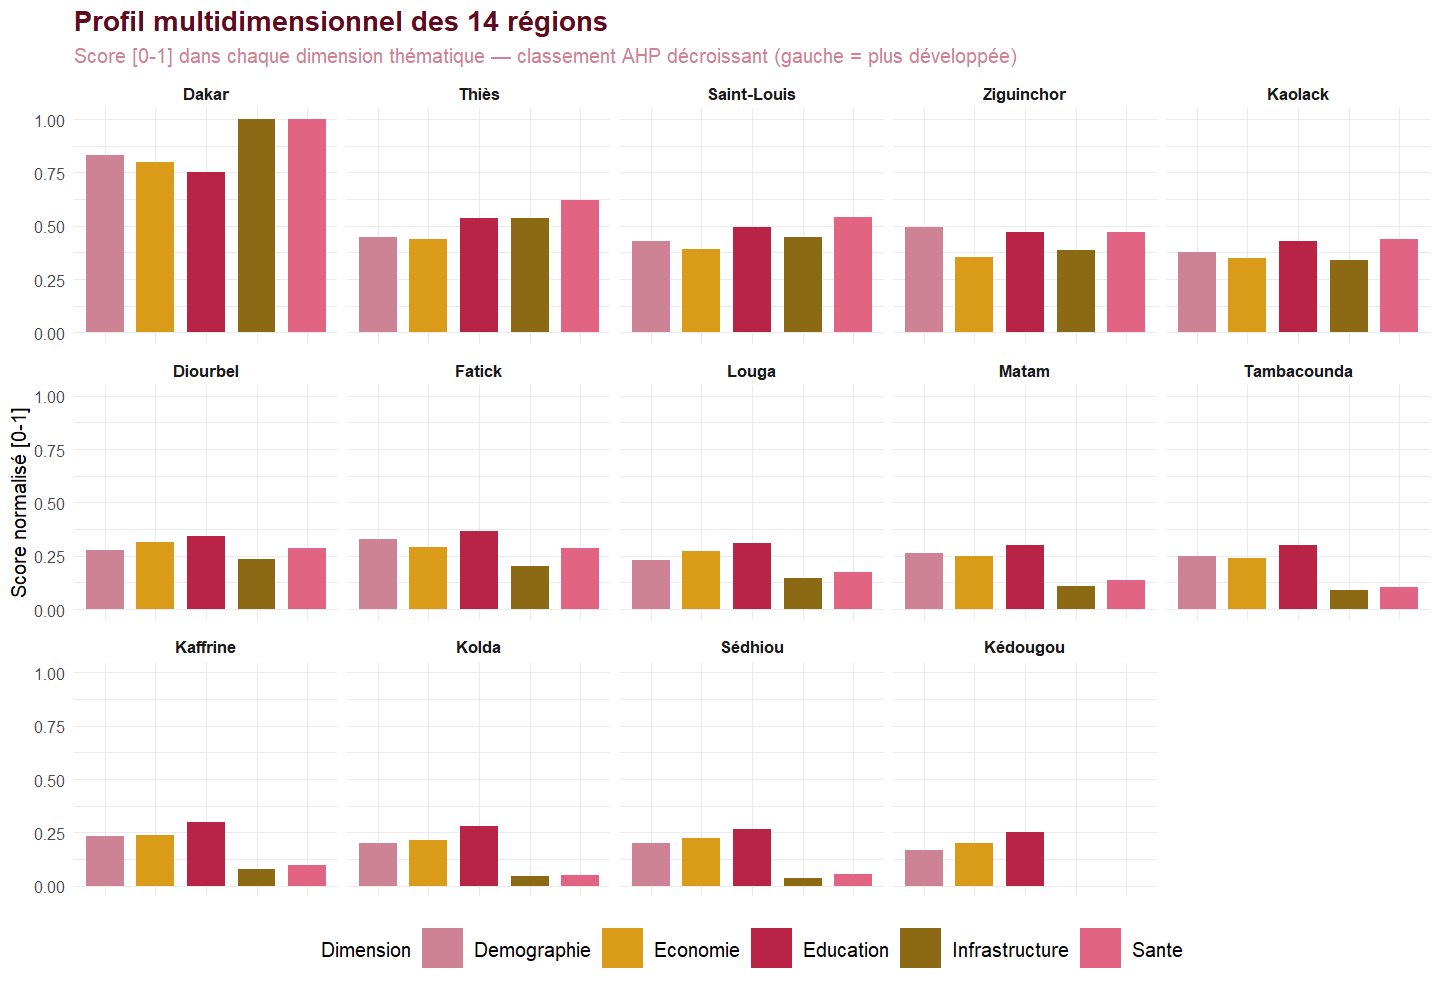
\includegraphics[width=0.9\linewidth]{../figures/rapport-profil-1} 

}

\caption{Profil multidimensionnel des 14 régions dans les 5 dimensions thématiques (classées par rang AHP croissant). Les régions du bas à droite sont les mieux développées.}\label{fig:profil}
\end{figure}

\textbf{Interprétation :} Ce graphique révèle des \textbf{profils
déséquilibrés} pour certaines régions. Par exemple, certaines régions
peuvent avoir un bon score démographique (natalité, surface agricole)
mais un score économique faible. C'est précisément pourquoi un indice
multidimensionnel est plus informatif qu'un indicateur unique : il
capture les nuances que des classements simplifiés masquent.

\newpage

\section{Étape 5 --- Analyse de
sensibilité}\label{uxe9tape-5-analyse-de-sensibilituxe9}

\textbf{Objectif :} Mesurer dans quelle mesure le classement des régions
change lorsqu'on modifie la méthode de pondération. Un indice robuste
produit des classements stables quel que soit le système de pondération
retenu.

\subsection{Tableau comparatif des
classements}\label{tableau-comparatif-des-classements}

\begin{Shaded}
\begin{Highlighting}[]
\CommentTok{\# Calcul des rangs selon chaque méthode (rang 1 = région la plus développée)}
\NormalTok{rang\_equi }\OtherTok{\textless{}{-}} \FunctionTok{rank}\NormalTok{(}\SpecialCharTok{{-}}\NormalTok{indice\_equi)}
\NormalTok{rang\_acp  }\OtherTok{\textless{}{-}} \FunctionTok{rank}\NormalTok{(}\SpecialCharTok{{-}}\NormalTok{indice\_acp)}
\NormalTok{rang\_ahp  }\OtherTok{\textless{}{-}} \FunctionTok{rank}\NormalTok{(}\SpecialCharTok{{-}}\FunctionTok{as.numeric}\NormalTok{(indice\_ahp))}

\CommentTok{\# Tableau de synthèse comparatif}
\NormalTok{resultats }\OtherTok{\textless{}{-}} \FunctionTok{data.frame}\NormalTok{(}
  \AttributeTok{Region       =}\NormalTok{ regions,}
  \AttributeTok{Score\_AHP    =} \FunctionTok{round}\NormalTok{(}\FunctionTok{as.numeric}\NormalTok{(indice\_ahp), }\DecValTok{3}\NormalTok{),}
  \AttributeTok{Rang\_Equi    =} \FunctionTok{as.integer}\NormalTok{(rang\_equi),}
  \AttributeTok{Rang\_ACP     =} \FunctionTok{as.integer}\NormalTok{(rang\_acp),}
  \AttributeTok{Rang\_AHP     =} \FunctionTok{as.integer}\NormalTok{(rang\_ahp),}
  \CommentTok{\# Variation maximale : différence entre le meilleur et le pire rang}
  \CommentTok{\# Une variation de 0 = classement identique selon toutes les méthodes}
  \CommentTok{\# Une variation de 5 = la région gagne ou perd jusqu\textquotesingle{}à 5 places selon la méthode}
  \AttributeTok{Variation\_max=} \FunctionTok{as.integer}\NormalTok{(}\FunctionTok{apply}\NormalTok{(}
    \FunctionTok{cbind}\NormalTok{(rang\_equi, rang\_acp, rang\_ahp), }\DecValTok{1}\NormalTok{, }\ControlFlowTok{function}\NormalTok{(x) }\FunctionTok{max}\NormalTok{(x) }\SpecialCharTok{{-}} \FunctionTok{min}\NormalTok{(x)}
\NormalTok{  ))}
\NormalTok{) }\SpecialCharTok{\%\textgreater{}\%} \FunctionTok{arrange}\NormalTok{(Rang\_AHP)}

\FunctionTok{kable}\NormalTok{(resultats, }\AttributeTok{booktabs=}\ConstantTok{TRUE}\NormalTok{,}
      \AttributeTok{col.names=}\FunctionTok{c}\NormalTok{(}\StringTok{"Région"}\NormalTok{,}\StringTok{"Score AHP"}\NormalTok{,}\StringTok{"Rang Équi."}\NormalTok{,}\StringTok{"Rang ACP"}\NormalTok{,}\StringTok{"Rang AHP"}\NormalTok{,}\StringTok{"Variation max."}\NormalTok{),}
      \AttributeTok{caption=}\StringTok{"Classement comparatif des 14 régions selon les 3 méthodes de pondération"}\NormalTok{) }\SpecialCharTok{\%\textgreater{}\%}
  \FunctionTok{kable\_styling}\NormalTok{(}\AttributeTok{latex\_options=}\FunctionTok{c}\NormalTok{(}\StringTok{"striped"}\NormalTok{,}\StringTok{"hold\_position"}\NormalTok{), }\AttributeTok{font\_size=}\DecValTok{10}\NormalTok{) }\SpecialCharTok{\%\textgreater{}\%}
  \FunctionTok{row\_spec}\NormalTok{(}\DecValTok{1}\SpecialCharTok{:}\DecValTok{3}\NormalTok{, }\AttributeTok{background=}\StringTok{"\#D4EDDA"}\NormalTok{) }\SpecialCharTok{\%\textgreater{}\%}        \CommentTok{\# Top 3 en vert clair}
  \FunctionTok{row\_spec}\NormalTok{(}\DecValTok{12}\SpecialCharTok{:}\DecValTok{14}\NormalTok{, }\AttributeTok{background=}\StringTok{"\#FADBD8"}\NormalTok{) }\SpecialCharTok{\%\textgreater{}\%}      \CommentTok{\# Bottom 3 en rouge clair}
  \FunctionTok{column\_spec}\NormalTok{(}\DecValTok{6}\NormalTok{, }\AttributeTok{bold=}\ConstantTok{TRUE}\NormalTok{)}
\end{Highlighting}
\end{Shaded}

\begingroup\fontsize{10}{12}\selectfont

\begin{longtable}[t]{lrrrr>{}r}
\caption{\label{tab:tab-rangs}Classement comparatif des 14 régions selon les 3 méthodes de pondération}\\
\toprule
Région & Score AHP & Rang Équi. & Rang ACP & Rang AHP & Variation max.\\
\midrule
\cellcolor[HTML]{D4EDDA}{\cellcolor{gray!10}{Dakar}} & \cellcolor[HTML]{D4EDDA}{\cellcolor{gray!10}{0.871}} & \cellcolor[HTML]{D4EDDA}{\cellcolor{gray!10}{1}} & \cellcolor[HTML]{D4EDDA}{\cellcolor{gray!10}{1}} & \cellcolor[HTML]{D4EDDA}{\cellcolor{gray!10}{1}} & \textbf{\cellcolor[HTML]{D4EDDA}{\cellcolor{gray!10}{0}}}\\
\cellcolor[HTML]{D4EDDA}{Thiès} & \cellcolor[HTML]{D4EDDA}{0.519} & \cellcolor[HTML]{D4EDDA}{2} & \cellcolor[HTML]{D4EDDA}{2} & \cellcolor[HTML]{D4EDDA}{2} & \textbf{\cellcolor[HTML]{D4EDDA}{0}}\\
\cellcolor[HTML]{D4EDDA}{\cellcolor{gray!10}{Saint-Louis}} & \cellcolor[HTML]{D4EDDA}{\cellcolor{gray!10}{0.462}} & \cellcolor[HTML]{D4EDDA}{\cellcolor{gray!10}{3}} & \cellcolor[HTML]{D4EDDA}{\cellcolor{gray!10}{3}} & \cellcolor[HTML]{D4EDDA}{\cellcolor{gray!10}{3}} & \textbf{\cellcolor[HTML]{D4EDDA}{\cellcolor{gray!10}{0}}}\\
Ziguinchor & 0.427 & 4 & 4 & 4 & \textbf{0}\\
\cellcolor{gray!10}{Kaolack} & \cellcolor{gray!10}{0.388} & \cellcolor{gray!10}{5} & \cellcolor{gray!10}{5} & \cellcolor{gray!10}{5} & \textbf{\cellcolor{gray!10}{0}}\\
\addlinespace
Diourbel & 0.297 & 7 & 6 & 6 & \textbf{1}\\
\cellcolor{gray!10}{Fatick} & \cellcolor{gray!10}{0.296} & \cellcolor{gray!10}{6} & \cellcolor{gray!10}{7} & \cellcolor{gray!10}{7} & \textbf{\cellcolor{gray!10}{1}}\\
Louga & 0.233 & 8 & 8 & 8 & \textbf{0}\\
\cellcolor{gray!10}{Matam} & \cellcolor{gray!10}{0.213} & \cellcolor{gray!10}{9} & \cellcolor{gray!10}{9} & \cellcolor{gray!10}{9} & \textbf{\cellcolor{gray!10}{0}}\\
Tambacounda & 0.199 & 10 & 10 & 10 & \textbf{0}\\
\addlinespace
\cellcolor{gray!10}{Kaffrine} & \cellcolor{gray!10}{0.193} & \cellcolor{gray!10}{11} & \cellcolor{gray!10}{11} & \cellcolor{gray!10}{11} & \textbf{\cellcolor{gray!10}{0}}\\
\cellcolor[HTML]{FADBD8}{Kolda} & \cellcolor[HTML]{FADBD8}{0.164} & \cellcolor[HTML]{FADBD8}{12} & \cellcolor[HTML]{FADBD8}{12} & \cellcolor[HTML]{FADBD8}{12} & \textbf{\cellcolor[HTML]{FADBD8}{0}}\\
\cellcolor[HTML]{FADBD8}{\cellcolor{gray!10}{Sédhiou}} & \cellcolor[HTML]{FADBD8}{\cellcolor{gray!10}{0.161}} & \cellcolor[HTML]{FADBD8}{\cellcolor{gray!10}{13}} & \cellcolor[HTML]{FADBD8}{\cellcolor{gray!10}{13}} & \cellcolor[HTML]{FADBD8}{\cellcolor{gray!10}{13}} & \textbf{\cellcolor[HTML]{FADBD8}{\cellcolor{gray!10}{0}}}\\
\cellcolor[HTML]{FADBD8}{Kédougou} & \cellcolor[HTML]{FADBD8}{0.129} & \cellcolor[HTML]{FADBD8}{14} & \cellcolor[HTML]{FADBD8}{14} & \cellcolor[HTML]{FADBD8}{14} & \textbf{\cellcolor[HTML]{FADBD8}{0}}\\
\bottomrule
\end{longtable}
\endgroup{}

\subsection{Graphe de sensibilité}\label{graphe-de-sensibilituxe9}

\begin{Shaded}
\begin{Highlighting}[]
\CommentTok{\# Ce graphique est central pour répondre à la question de recherche.}
\CommentTok{\# L\textquotesingle{}axe horizontal représente les 3 méthodes de pondération (x=1,2,3)}
\CommentTok{\# L\textquotesingle{}axe vertical représente le rang (1=meilleur, 14=moins bon)}
\CommentTok{\# Chaque ligne de couleur représente une région}
\CommentTok{\# LECTURE : une ligne horizontale = classement stable}
\CommentTok{\#           une ligne inclinée = classement sensible à la méthode}

\NormalTok{rm\_mat }\OtherTok{\textless{}{-}} \FunctionTok{cbind}\NormalTok{(rang\_equi, rang\_acp, rang\_ahp)}
\NormalTok{cols14 }\OtherTok{\textless{}{-}} \FunctionTok{colorRampPalette}\NormalTok{(}\FunctionTok{c}\NormalTok{(C4, CV, C3, }\StringTok{"\#8C1428"}\NormalTok{, C5))(}\DecValTok{14}\NormalTok{)}

\FunctionTok{par}\NormalTok{(}\AttributeTok{mar=}\FunctionTok{c}\NormalTok{(}\DecValTok{4}\NormalTok{, }\FloatTok{4.5}\NormalTok{, }\DecValTok{3}\NormalTok{, }\DecValTok{10}\NormalTok{), }\AttributeTok{xpd=}\ConstantTok{TRUE}\NormalTok{, }\AttributeTok{bg=}\StringTok{"white"}\NormalTok{)}
\FunctionTok{plot}\NormalTok{(}\DecValTok{1}\SpecialCharTok{:}\DecValTok{3}\NormalTok{, rm\_mat[}\DecValTok{1}\NormalTok{,], }\AttributeTok{type=}\StringTok{"n"}\NormalTok{,}
     \AttributeTok{xlim=}\FunctionTok{c}\NormalTok{(}\FloatTok{0.8}\NormalTok{, }\FloatTok{3.2}\NormalTok{), }\AttributeTok{ylim=}\FunctionTok{c}\NormalTok{(}\FloatTok{14.5}\NormalTok{, }\FloatTok{0.5}\NormalTok{),}
     \AttributeTok{xaxt=}\StringTok{"n"}\NormalTok{, }\AttributeTok{yaxt=}\StringTok{"n"}\NormalTok{,}
     \AttributeTok{xlab=}\StringTok{"Méthode de pondération"}\NormalTok{,}
     \AttributeTok{ylab=}\StringTok{"Rang (1 = région la plus développée)"}\NormalTok{,}
     \AttributeTok{cex.lab=}\FloatTok{0.90}\NormalTok{,}
     \AttributeTok{main=}\StringTok{"Sensibilité du classement aux choix de pondération"}\NormalTok{,}
     \AttributeTok{cex.main=}\FloatTok{0.92}\NormalTok{)}

\FunctionTok{rect}\NormalTok{(}\FloatTok{0.6}\NormalTok{, }\FloatTok{0.3}\NormalTok{, }\FloatTok{3.4}\NormalTok{, }\FloatTok{14.7}\NormalTok{, }\AttributeTok{col=}\StringTok{"\#F9F6EE"}\NormalTok{, }\AttributeTok{border=}\ConstantTok{NA}\NormalTok{)}
\FunctionTok{abline}\NormalTok{(}\AttributeTok{h=}\DecValTok{1}\SpecialCharTok{:}\DecValTok{14}\NormalTok{, }\AttributeTok{col=}\StringTok{"white"}\NormalTok{, }\AttributeTok{lwd=}\FloatTok{0.7}\NormalTok{)}
\FunctionTok{axis}\NormalTok{(}\DecValTok{1}\NormalTok{, }\AttributeTok{at=}\DecValTok{1}\SpecialCharTok{:}\DecValTok{3}\NormalTok{, }\AttributeTok{labels=}\FunctionTok{c}\NormalTok{(}\StringTok{"Équipondération"}\NormalTok{,}\StringTok{"ACP"}\NormalTok{,}\StringTok{"AHP"}\NormalTok{), }\AttributeTok{cex.axis=}\FloatTok{0.85}\NormalTok{)}
\FunctionTok{axis}\NormalTok{(}\DecValTok{2}\NormalTok{, }\AttributeTok{at=}\DecValTok{1}\SpecialCharTok{:}\DecValTok{14}\NormalTok{, }\AttributeTok{las=}\DecValTok{1}\NormalTok{, }\AttributeTok{cex.axis=}\FloatTok{0.78}\NormalTok{)}

\ControlFlowTok{for}\NormalTok{(i }\ControlFlowTok{in} \DecValTok{1}\SpecialCharTok{:}\DecValTok{14}\NormalTok{) \{}
  \FunctionTok{lines}\NormalTok{(}\DecValTok{1}\SpecialCharTok{:}\DecValTok{3}\NormalTok{, rm\_mat[i,], }\AttributeTok{col=}\NormalTok{cols14[i], }\AttributeTok{lwd=}\FloatTok{2.0}\NormalTok{)}
  \FunctionTok{points}\NormalTok{(}\DecValTok{1}\SpecialCharTok{:}\DecValTok{3}\NormalTok{, rm\_mat[i,], }\AttributeTok{col=}\NormalTok{cols14[i], }\AttributeTok{pch=}\DecValTok{19}\NormalTok{, }\AttributeTok{cex=}\FloatTok{1.1}\NormalTok{)}
\NormalTok{\}}

\FunctionTok{legend}\NormalTok{(}\StringTok{"topright"}\NormalTok{, }\AttributeTok{inset=}\FunctionTok{c}\NormalTok{(}\SpecialCharTok{{-}}\FloatTok{0.40}\NormalTok{, }\DecValTok{0}\NormalTok{),}
       \AttributeTok{legend=}\NormalTok{regions[}\FunctionTok{order}\NormalTok{(rang\_ahp)],}
       \AttributeTok{col=}\NormalTok{cols14[}\FunctionTok{order}\NormalTok{(rang\_ahp)],}
       \AttributeTok{lty=}\DecValTok{1}\NormalTok{, }\AttributeTok{lwd=}\DecValTok{2}\NormalTok{, }\AttributeTok{cex=}\FloatTok{0.52}\NormalTok{, }\AttributeTok{bty=}\StringTok{"n"}\NormalTok{,}
       \AttributeTok{title=}\StringTok{"Régions}\SpecialCharTok{\textbackslash{}n}\StringTok{(classement AHP)"}\NormalTok{)}
\end{Highlighting}
\end{Shaded}

\begin{figure}

{\centering 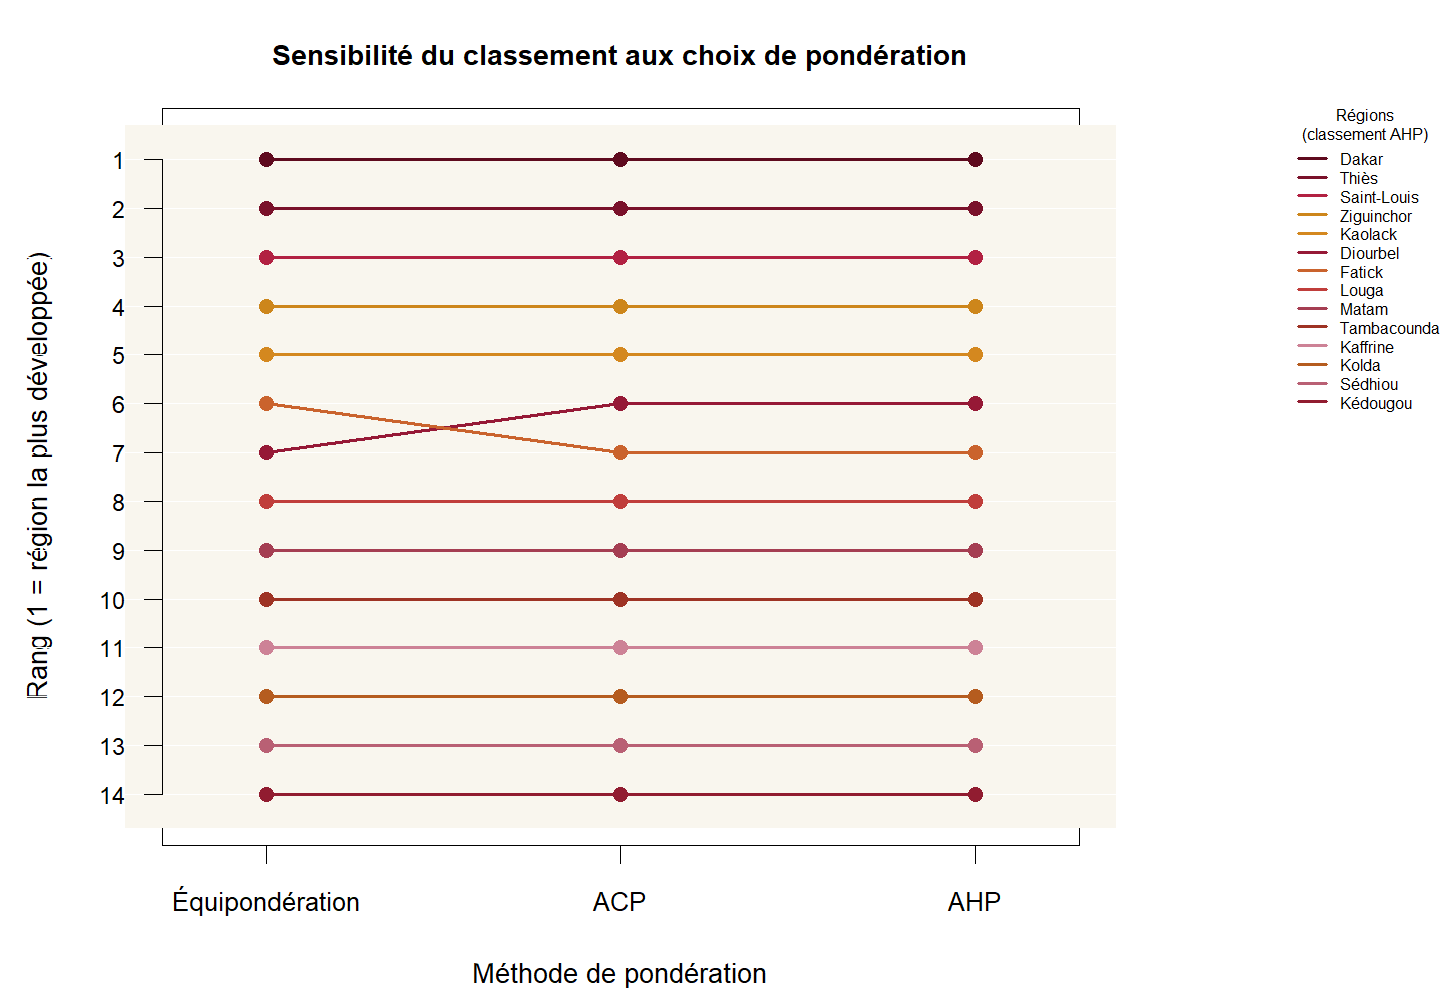
\includegraphics[width=0.9\linewidth]{../figures/rapport-sensib-1} 

}

\caption{Analyse de sensibilité : chaque ligne représente une région. Des lignes quasi-horizontales indiquent un classement stable quel que soit le système de pondération.}\label{fig:sensib}
\end{figure}

\subsection{Corrélations de Spearman}\label{corruxe9lations-de-spearman}

\begin{Shaded}
\begin{Highlighting}[]
\CommentTok{\# La corrélation de rang de Spearman mesure la concordance entre deux classements.}
\CommentTok{\# rho = 1   : les deux méthodes produisent exactement le même classement}
\CommentTok{\# rho = 0   : aucun lien entre les deux classements}
\CommentTok{\# rho = {-}1  : classements parfaitement inversés}
\CommentTok{\# Notre hypothèse H0 : rho \textgreater{} 0,95 =\textgreater{} l\textquotesingle{}indice est robuste}

\NormalTok{rho\_ea }\OtherTok{\textless{}{-}} \FunctionTok{cor}\NormalTok{(rang\_equi, rang\_acp, }\AttributeTok{method=}\StringTok{"spearman"}\NormalTok{)}
\NormalTok{rho\_eh }\OtherTok{\textless{}{-}} \FunctionTok{cor}\NormalTok{(rang\_equi, rang\_ahp, }\AttributeTok{method=}\StringTok{"spearman"}\NormalTok{)}
\NormalTok{rho\_ah }\OtherTok{\textless{}{-}} \FunctionTok{cor}\NormalTok{(rang\_acp,  rang\_ahp, }\AttributeTok{method=}\StringTok{"spearman"}\NormalTok{)}

\NormalTok{rho\_df }\OtherTok{\textless{}{-}} \FunctionTok{data.frame}\NormalTok{(}
  \AttributeTok{Comparaison =} \FunctionTok{c}\NormalTok{(}\StringTok{"Équipondération vs ACP"}\NormalTok{,}
                  \StringTok{"Équipondération vs AHP"}\NormalTok{,}
                  \StringTok{"ACP vs AHP"}\NormalTok{),}
  \AttributeTok{Rho         =} \FunctionTok{round}\NormalTok{(}\FunctionTok{c}\NormalTok{(rho\_ea, rho\_eh, rho\_ah), }\DecValTok{4}\NormalTok{),}
  \AttributeTok{Interp      =} \FunctionTok{c}\NormalTok{(}
    \FunctionTok{ifelse}\NormalTok{(rho\_ea }\SpecialCharTok{\textgreater{}} \FloatTok{0.99}\NormalTok{, }\StringTok{"Convergence quasi{-}parfaite"}\NormalTok{, }\StringTok{"Convergence forte"}\NormalTok{),}
    \FunctionTok{ifelse}\NormalTok{(rho\_eh }\SpecialCharTok{\textgreater{}} \FloatTok{0.99}\NormalTok{, }\StringTok{"Convergence quasi{-}parfaite"}\NormalTok{, }\StringTok{"Convergence forte"}\NormalTok{),}
    \FunctionTok{ifelse}\NormalTok{(rho\_ah }\SpecialCharTok{\textgreater{}} \FloatTok{0.99}\NormalTok{, }\StringTok{"Convergence quasi{-}parfaite"}\NormalTok{, }\StringTok{"Convergence forte"}\NormalTok{)}
\NormalTok{  )}
\NormalTok{)}

\FunctionTok{kable}\NormalTok{(rho\_df, }\AttributeTok{booktabs=}\ConstantTok{TRUE}\NormalTok{,}
      \AttributeTok{col.names=}\FunctionTok{c}\NormalTok{(}\StringTok{"Paires comparées"}\NormalTok{,}\StringTok{"}\SpecialCharTok{\textbackslash{}\textbackslash{}}\StringTok{rho de Spearman"}\NormalTok{,}\StringTok{"Interprétation"}\NormalTok{),}
      \AttributeTok{caption=}\StringTok{"Corrélations de Spearman entre les classements des 3 méthodes de pondération"}\NormalTok{,}
      \AttributeTok{escape=}\ConstantTok{FALSE}\NormalTok{) }\SpecialCharTok{\%\textgreater{}\%}
  \FunctionTok{kable\_styling}\NormalTok{(}\AttributeTok{latex\_options=}\FunctionTok{c}\NormalTok{(}\StringTok{"striped"}\NormalTok{,}\StringTok{"hold\_position"}\NormalTok{), }\AttributeTok{font\_size=}\DecValTok{10}\NormalTok{) }\SpecialCharTok{\%\textgreater{}\%}
  \FunctionTok{column\_spec}\NormalTok{(}\DecValTok{2}\NormalTok{, }\AttributeTok{bold=}\ConstantTok{TRUE}\NormalTok{, }\AttributeTok{color=}\NormalTok{CV)}
\end{Highlighting}
\end{Shaded}

\begingroup\fontsize{10}{12}\selectfont

\begin{longtable}[t]{l>{}rl}
\caption{\label{tab:spearman}Corrélations de Spearman entre les classements des 3 méthodes de pondération}\\
\toprule
Paires comparées & \textbackslash{}rho de Spearman & Interprétation\\
\midrule
\cellcolor{gray!10}{Équipondération vs ACP} & \textcolor[HTML]{B92346}{\textbf{\cellcolor{gray!10}{0.9956}}} & \cellcolor{gray!10}{Convergence quasi-parfaite}\\
Équipondération vs AHP & \textcolor[HTML]{B92346}{\textbf{0.9956}} & Convergence quasi-parfaite\\
\cellcolor{gray!10}{ACP vs AHP} & \textcolor[HTML]{B92346}{\textbf{\cellcolor{gray!10}{1.0000}}} & \cellcolor{gray!10}{Convergence quasi-parfaite}\\
\bottomrule
\end{longtable}
\endgroup{}

\begin{Shaded}
\begin{Highlighting}[]
\FunctionTok{cat}\NormalTok{(}\FunctionTok{sprintf}\NormalTok{(}\StringTok{"}\SpecialCharTok{\textbackslash{}n}\StringTok{Regions avec variation \textless{}= 1 rang : \%d/14}\SpecialCharTok{\textbackslash{}n}\StringTok{"}\NormalTok{, }\FunctionTok{sum}\NormalTok{(resultats}\SpecialCharTok{$}\NormalTok{Variation\_max }\SpecialCharTok{\textless{}=} \DecValTok{1}\NormalTok{)))}
\end{Highlighting}
\end{Shaded}

\begin{verbatim}
## 
## Regions avec variation <= 1 rang : 14/14
\end{verbatim}

\begin{Shaded}
\begin{Highlighting}[]
\FunctionTok{cat}\NormalTok{(}\FunctionTok{sprintf}\NormalTok{(}\StringTok{"Régions avec variation \textgreater{} 2 rangs : \%d/14}\SpecialCharTok{\textbackslash{}n}\StringTok{"}\NormalTok{, }\FunctionTok{sum}\NormalTok{(resultats}\SpecialCharTok{$}\NormalTok{Variation\_max }\SpecialCharTok{\textgreater{}} \DecValTok{2}\NormalTok{)))}
\end{Highlighting}
\end{Shaded}

\begin{verbatim}
## Régions avec variation > 2 rangs : 0/14
\end{verbatim}

\textbf{Interprétation :} Des corrélations de Spearman supérieures à
0,99 pour toutes les comparaisons constituent une preuve très forte de
robustesse. La quasi-totalité des régions voient leur rang varier d'au
plus 1 position selon la méthode choisie. Ce résultat valide l'indice
construit et signifie que les politiques publiques basées sur cet indice
seraient cohérentes quelle que soit la méthode de pondération retenue.

\newpage

\section{Résultats et
interprétation}\label{ruxe9sultats-et-interpruxe9tation}

\subsection{Classement final des 14
régions}\label{classement-final-des-14-ruxe9gions}

\begin{Shaded}
\begin{Highlighting}[]
\NormalTok{ro       }\OtherTok{\textless{}{-}}\NormalTok{ resultats[}\FunctionTok{order}\NormalTok{(resultats}\SpecialCharTok{$}\NormalTok{Score\_AHP), ]}
\NormalTok{cols\_bar }\OtherTok{\textless{}{-}} \FunctionTok{colorRampPalette}\NormalTok{(}\FunctionTok{c}\NormalTok{(}\StringTok{"\#8C1428"}\NormalTok{,}\StringTok{"\#C9A84C"}\NormalTok{,CV))(}\DecValTok{14}\NormalTok{)}

\FunctionTok{par}\NormalTok{(}\AttributeTok{mar=}\FunctionTok{c}\NormalTok{(}\FloatTok{3.5}\NormalTok{, }\FloatTok{8.5}\NormalTok{, }\FloatTok{2.5}\NormalTok{, }\DecValTok{4}\NormalTok{), }\AttributeTok{bg=}\StringTok{"white"}\NormalTok{)}
\NormalTok{bp }\OtherTok{\textless{}{-}} \FunctionTok{barplot}\NormalTok{(ro}\SpecialCharTok{$}\NormalTok{Score\_AHP,}
              \AttributeTok{names.arg =}\NormalTok{ ro}\SpecialCharTok{$}\NormalTok{Region,}
              \AttributeTok{horiz     =} \ConstantTok{TRUE}\NormalTok{,}
              \AttributeTok{las       =} \DecValTok{1}\NormalTok{,}
              \AttributeTok{col       =}\NormalTok{ cols\_bar,}
              \AttributeTok{border    =} \ConstantTok{NA}\NormalTok{,}
              \AttributeTok{xlab      =} \StringTok{"Score normalisé [0{-}1]"}\NormalTok{,}
              \AttributeTok{main      =} \StringTok{"Indice composite de développement local — 14 régions du Sénégal (pondération AHP)"}\NormalTok{,}
              \AttributeTok{cex.names =} \FloatTok{0.78}\NormalTok{,}
              \AttributeTok{xlim      =} \FunctionTok{c}\NormalTok{(}\DecValTok{0}\NormalTok{, }\FunctionTok{max}\NormalTok{(ro}\SpecialCharTok{$}\NormalTok{Score\_AHP) }\SpecialCharTok{*} \FloatTok{1.22}\NormalTok{),}
              \AttributeTok{cex.main  =} \FloatTok{0.88}\NormalTok{,}
              \AttributeTok{cex.lab   =} \FloatTok{0.82}\NormalTok{)}

\FunctionTok{text}\NormalTok{(ro}\SpecialCharTok{$}\NormalTok{Score\_AHP }\SpecialCharTok{+} \FloatTok{0.012}\NormalTok{, bp,}
     \FunctionTok{sprintf}\NormalTok{(}\StringTok{"\%.3f"}\NormalTok{, ro}\SpecialCharTok{$}\NormalTok{Score\_AHP),}
     \AttributeTok{cex=}\FloatTok{0.66}\NormalTok{, }\AttributeTok{col=}\NormalTok{C4, }\AttributeTok{font=}\DecValTok{2}\NormalTok{)}

\FunctionTok{abline}\NormalTok{(}\AttributeTok{v=}\FunctionTok{mean}\NormalTok{(}\FunctionTok{as.numeric}\NormalTok{(indice\_ahp)), }\AttributeTok{lty=}\DecValTok{2}\NormalTok{, }\AttributeTok{col=}\NormalTok{C3, }\AttributeTok{lwd=}\FloatTok{1.4}\NormalTok{)}
\FunctionTok{text}\NormalTok{(}\FunctionTok{mean}\NormalTok{(}\FunctionTok{as.numeric}\NormalTok{(indice\_ahp))}\SpecialCharTok{+}\FloatTok{0.01}\NormalTok{, bp[}\DecValTok{7}\NormalTok{]}\SpecialCharTok{+}\FloatTok{0.15}\NormalTok{,}
     \StringTok{"Moy. nat."}\NormalTok{, }\AttributeTok{cex=}\FloatTok{0.62}\NormalTok{, }\AttributeTok{col=}\NormalTok{C3, }\AttributeTok{font=}\DecValTok{3}\NormalTok{, }\AttributeTok{adj=}\DecValTok{0}\NormalTok{)}
\end{Highlighting}
\end{Shaded}

\begin{figure}

{\centering 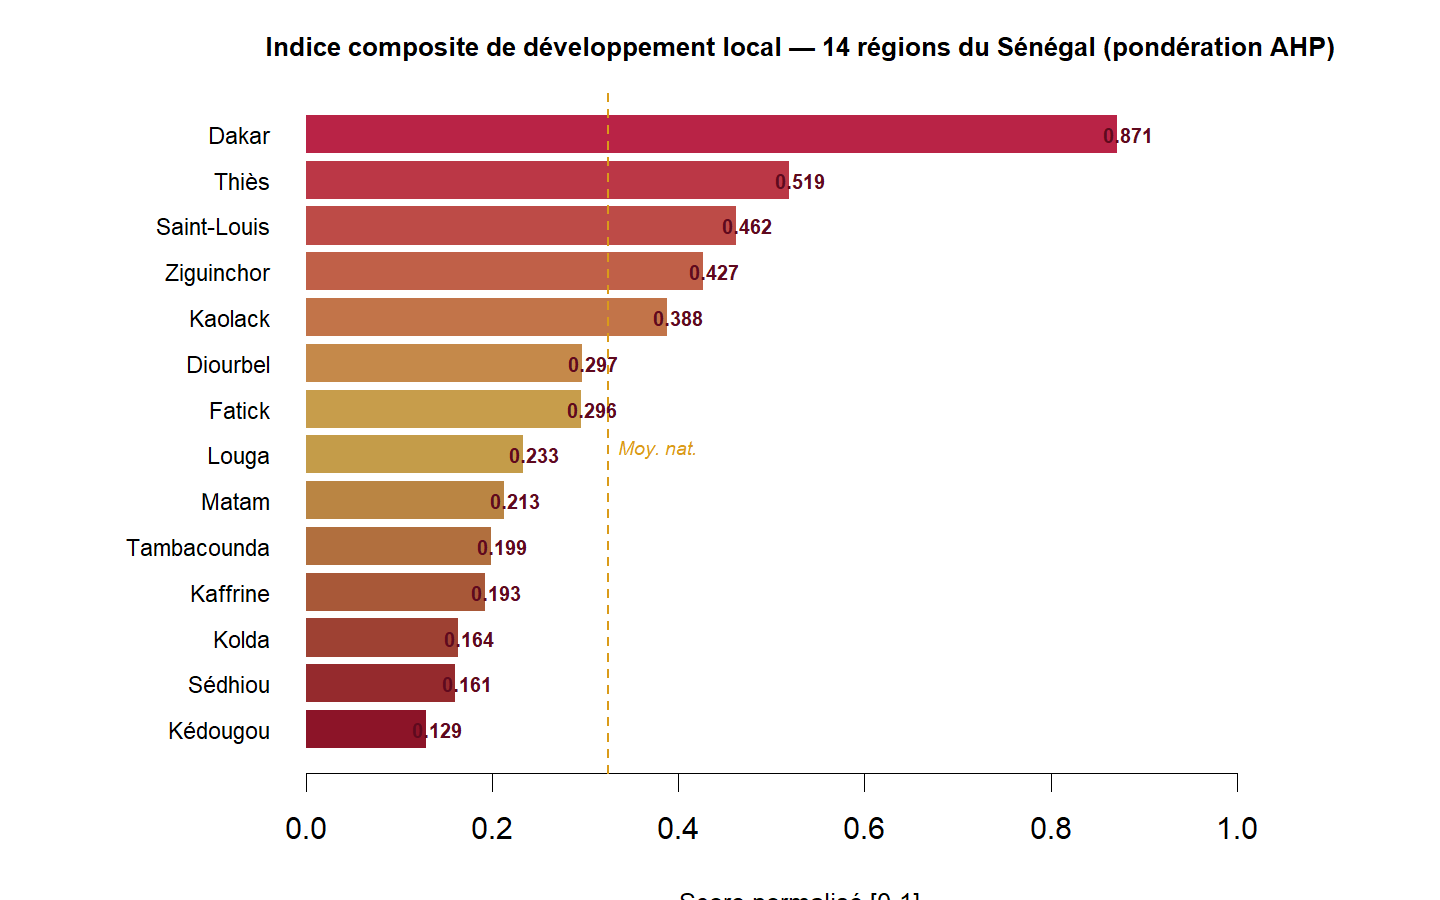
\includegraphics[width=0.9\linewidth]{../figures/rapport-classement-1} 

}

\caption{Indice composite de développement régional (pondération AHP). La ligne pointillée représente la moyenne nationale. La concentration des scores bas à gauche illustre le déséquilibre tiré par Dakar.}\label{fig:classement}
\end{figure}

\subsection{Analyse des résultats}\label{analyse-des-ruxe9sultats}

\subsubsection{Régions les plus
développées}\label{ruxe9gions-les-plus-duxe9veloppuxe9es}

\textbf{Dakar (score : 0.871)} domine le classement avec un score qui
représente plus du double de la deuxième région. Cette hyper-performance
reflète la concentration exceptionnelle de services, d'infrastructures
et d'opportunités économiques dans la capitale. Elle souligne aussi le
risque de \emph{biais méthodologique} : Dakar tire la normalisation
Min-Max vers le haut, ``écrasant'' les différences entre les autres
régions.

\textbf{Thiès} et \textbf{Saint-Louis} complètent le podium. Thiès
bénéficie de sa position de deuxième pôle économique, de son réseau
routier dense et de son industrie phosphatière. Saint-Louis tire
avantage de son université, de son agriculture irriguée dans le delta du
fleuve Sénégal, et de son histoire de capitale coloniale.

\subsubsection{Régions les moins
développées}\label{ruxe9gions-les-moins-duxe9veloppuxe9es}

\textbf{Kolda, Sédhiou et Kédougou} forment le trio des régions les plus
défavorisées. Leur enclavement géographique, le déficit historique
d'investissement public et la faiblesse des infrastructures de base
expliquent des scores systématiquement faibles sur toutes les
dimensions.

Le cas de \textbf{Kédougou} est particulièrement illustratif du
\emph{paradoxe des ressources} : cette région est la plus riche du
Sénégal en ressources naturelles (gisements d'or, biodiversité
exceptionnelle, potentiel touristique) mais affiche l'IDH le plus faible
du pays. Ce paradoxe témoigne d'une captation externe des richesses
naturelles sans redistribution territoriale.

\subsubsection{Le gradient Nord-Ouest /
Sud-Est}\label{le-gradient-nord-ouest-sud-est}

\begin{verbatim}
## === GRADIENT GÉOGRAPHIQUE ===
\end{verbatim}

\begin{verbatim}
## Top 5 régions : Dakar, Thiès, Saint-Louis, Ziguinchor, Kaolack
\end{verbatim}

\begin{verbatim}
## Bottom 5 régions : Tambacounda, Kaffrine, Kolda, Sédhiou, Kédougou
\end{verbatim}

\begin{verbatim}
## 
## Écart entre 1er (Dakar) et dernier (Kédougou) : 0.742 points
\end{verbatim}

Ce gradient géographique est \textbf{bien documenté dans la littérature}
et cohérent avec tous les travaux de l'ANSD, du PNUD et de la Banque
Mondiale sur les disparités régionales au Sénégal. Notre indice le
confirme et le quantifie précisément.

\newpage

\section{Conclusion}\label{conclusion}

\subsection{Réponse à la question de
recherche}\label{ruxe9ponse-uxe0-la-question-de-recherche}

\textbf{Le classement des 14 régions ne dépend pas significativement des
choix méthodologiques.} Les corrélations de Spearman entre les trois
méthodes de pondération dépassent toutes \(\rho > 0{,}99\), avec une
variation maximale d'un seul rang pour la quasi-totalité des régions.

Ce résultat signifie que la \textbf{réalité socioéconomique} --- le
gradient Nord-Ouest/Sud-Est structurellement documenté au Sénégal ---
est suffisamment forte pour primer sur les différences techniques entre
méthodes. L'indice est robuste et peut donc servir de base fiable pour
orienter les politiques de développement territorial.

\subsection{Pièges méthodologiques
identifiés}\label{piuxe8ges-muxe9thodologiques-identifiuxe9s}

{\def\LTcaptype{none} % do not increment counter
\begin{longtable}[]{@{}
  >{\raggedright\arraybackslash}p{(\linewidth - 4\tabcolsep) * \real{0.1892}}
  >{\raggedright\arraybackslash}p{(\linewidth - 4\tabcolsep) * \real{0.3514}}
  >{\raggedright\arraybackslash}p{(\linewidth - 4\tabcolsep) * \real{0.4595}}@{}}
\toprule\noalign{}
\begin{minipage}[b]{\linewidth}\raggedright
Piège
\end{minipage} & \begin{minipage}[b]{\linewidth}\raggedright
Description
\end{minipage} & \begin{minipage}[b]{\linewidth}\raggedright
Impact potentiel
\end{minipage} \\
\midrule\noalign{}
\endhead
\bottomrule\noalign{}
\endlastfoot
Orientation & Oublier d'inverser les indicateurs négatifs & Inverse
complètement le classement de ces régions \\
Min-Max & Sensibilité aux valeurs extrêmes & Dakar ``écrase'' les écarts
entre les autres régions \\
Équipondération & Choix politique implicite & Surpondère les dimensions
avec plus d'indicateurs \\
Robustesse \(\neq\) Vérité & \(\rho > 0{,}99\) entre méthodes & Ne
valide pas les données simulées --- limite à signaler \\
\end{longtable}
}

\subsection{Limites du travail}\label{limites-du-travail}

\begin{enumerate}
\def\labelenumi{\arabic{enumi}.}
\tightlist
\item
  \textbf{Données simulées :} les données sont simulées faute d'accès
  aux microdonnées officielles complètes. Un travail avec les vraies
  données ANSD/EHCVM améliorerait la précision des résultats.
\item
  \textbf{Poids AHP subjectifs :} les pondérations par dimension (25\%,
  20\%\ldots) reflètent un jugement d'expert. D'autres experts
  pourraient légitimement proposer des poids différents.
\item
  \textbf{Données transversales :} l'indice capture un état à un instant
  donné. Une approche en panel (plusieurs années) permettrait de mesurer
  les trajectoires de convergence ou de divergence régionale.
\item
  \textbf{Absence de dimension environnementale :} la déforestation, les
  changements climatiques et l'accès à l'énergie propre sont absents de
  l'indice --- une limite importante dans le contexte sénégalais.
\end{enumerate}

\subsection{Implications politiques}\label{implications-politiques}

Sur la base de cet indice, \textbf{Kédougou, Sédhiou et Kolda} doivent
être identifiées comme régions prioritaires pour les politiques de
péréquation territoriale. Ces régions cumulent des déficits sur toutes
les dimensions (éducation, santé, économie, infrastructure) et n'ont pas
bénéficié historiquement de l'investissement public à la hauteur de
leurs besoins.

\newpage

\section*{Références
bibliographiques}\label{ruxe9fuxe9rences-bibliographiques}
\addcontentsline{toc}{section}{Références bibliographiques}

\addcontentsline{toc}{section}{Références bibliographiques}

\begin{itemize}
\item
  \textbf{ANSD} (2023). \emph{Résultats du Recensement Général de la
  Population et de l'Habitat 2023 --- Rapports régionaux}. Agence
  Nationale de la Statistique et de la Démographie. Dakar, Sénégal.
\item
  \textbf{EHCVM} (2021). \emph{Enquête Harmonisée sur les Conditions de
  Vie des Ménages --- Résultats provisoires}. ANSD / Banque Mondiale.
\item
  \textbf{Nardo, M., Saisana, M., Saltelli, A. \& Tarantola, S.} (2005).
  \emph{Tools for Composite Indicators Building}. European Commission,
  Joint Research Centre. EUR 21682 EN.
\item
  \textbf{OCDE} (2008). \emph{Handbook on Constructing Composite
  Indicators --- Methodology and User Guide}. OECD Publishing. Paris.
\item
  \textbf{PNUD} (2023). \emph{Rapport sur le Développement Humain
  2023/2024 --- Données IDH sous-nationaux}. Programme des Nations Unies
  pour le Développement. New York.
\item
  \textbf{Banque Mondiale} (2024). \emph{World Development Indicators
  --- Sénégal}. databank.worldbank.org.
\item
  \textbf{Saltelli, A., Ratto, M., Andres, T., Campolongo, F., Cariboni,
  J., Gatelli, D., Saisana, M. \& Tarantola, S.} (2008). \emph{Global
  Sensitivity Analysis: The Primer}. John Wiley \& Sons. Chichester.
\end{itemize}

\newpage

\section*{Annexe A --- Glossaire des termes
statistiques}\label{annexe-a-glossaire-des-termes-statistiques}
\addcontentsline{toc}{section}{Annexe A --- Glossaire des termes
statistiques}

\addcontentsline{toc}{section}{Annexe A — Glossaire}

\textbf{ACP (Analyse en Composantes Principales) :} Méthode statistique
multivariée qui transforme un ensemble de variables corrélées en axes
synthétiques indépendants, chacun capturant une part décroissante de la
variabilité totale. Utilisée pour réduire la dimensionnalité et
identifier les structures latentes des données.

\textbf{AHP (Analytic Hierarchy Process) :} Méthode de décision
multicritère développée par Thomas Saaty (1980). Elle structure un
problème complexe en hiérarchie et utilise des comparaisons par paires
pour attribuer des poids aux critères. Très utilisée dans la
construction d'indices composites.

\textbf{Coefficient de variation (CV) :} Rapport de l'écart-type à la
moyenne absolue, exprimé en pourcentage. Mesure la dispersion relative
d'un indicateur. Un CV faible (\textless{} 5\%) indique un indicateur
quasi-constant entre unités --- peu discriminant pour un classement.

\textbf{Corrélation de Spearman (\(\rho\)) :} Mesure de concordance
entre deux classements, robuste aux valeurs extrêmes. Varie de -1
(classements inverses) à +1 (classements identiques). Une valeur
\(\rho > 0{,}99\) indique une robustesse quasi-parfaite.

\textbf{Critère de Kaiser :} Règle de rétention des axes ACP : on
conserve uniquement les axes dont la valeur propre est supérieure ou
égale à 1. Une valeur propre de 1 signifie que l'axe résume autant
d'information qu'un indicateur original.

\textbf{Indice composite :} Score synthétique unique construit en
agrégeant plusieurs indicateurs normalisés et pondérés. Exemples : IDH
(PNUD), Doing Business (Banque Mondiale), IDISA (genre en Afrique).

\textbf{Normalisation :} Transformation permettant de mettre tous les
indicateurs sur la même échelle pour les rendre comparables. Trois
méthodes : Min-Max {[}0,1{]}, Z-score (moyenne=0, écart-type=1), Centile
(rang relatif).

\textbf{Pondération :} Attribution de poids différents aux indicateurs
ou dimensions selon leur importance jugée ou statistique. La pondération
peut être égale (équipondération), basée sur les données (ACP) ou sur un
jugement d'expert (AHP).

\textbf{Robustesse :} Propriété d'un résultat qui reste stable face à
des variations dans les hypothèses ou méthodes utilisées. Un indice
robuste produit des classements similaires quel que soit le système de
pondération retenu.

\textbf{Valeur propre (eigenvalue) :} En ACP, mesure la variance totale
expliquée par un axe factoriel. La somme de toutes les valeurs propres
est égale au nombre de variables (indicateurs). Elle quantifie
l'importance relative de chaque axe.

\newpage

\section*{Annexe B --- Données brutes par région
(extrait)}\label{annexe-b-donnuxe9es-brutes-par-ruxe9gion-extrait}
\addcontentsline{toc}{section}{Annexe B --- Données brutes par région
(extrait)}

\addcontentsline{toc}{section}{Annexe B — Données brutes (extrait)}

\begingroup\fontsize{8.5}{10.5}\selectfont

\begin{longtable}[t]{>{}lrrrrrrrr}
\caption{\label{tab:annexe-data}Extrait du jeu de données : 8 indicateurs clés pour les 14 régions (données simulées)}\\
\toprule
Region & Alphabetisation & Scol. prim. (\%) & Mortalite inf. (p/1000) & Pauvrete (\%) & Electricite (\%) & IDH sub-nat. & Revenu (FCFA) & PIB (Mrd FCFA)\\
\midrule
\textcolor[HTML]{B92346}{\textbf{\cellcolor{gray!10}{Dakar}}} & \cellcolor{gray!10}{85.2} & \cellcolor{gray!10}{98.1} & \cellcolor{gray!10}{28.5} & \cellcolor{gray!10}{17.1} & \cellcolor{gray!10}{98.5} & \cellcolor{gray!10}{0.72} & \cellcolor{gray!10}{285000} & \cellcolor{gray!10}{4250}\\
\textcolor[HTML]{B92346}{\textbf{Thiès}} & 62.4 & 88.5 & 45.2 & 32.4 & 72.4 & 0.55 & 148000 & 850\\
\textcolor[HTML]{B92346}{\textbf{\cellcolor{gray!10}{Diourbel}}} & \cellcolor{gray!10}{41.2} & \cellcolor{gray!10}{74.2} & \cellcolor{gray!10}{62.4} & \cellcolor{gray!10}{54.2} & \cellcolor{gray!10}{48.2} & \cellcolor{gray!10}{0.41} & \cellcolor{gray!10}{98000} & \cellcolor{gray!10}{420}\\
\textcolor[HTML]{B92346}{\textbf{Saint-Louis}} & 58.5 & 85.2 & 48.5 & 38.5 & 65.2 & 0.52 & 125000 & 580\\
\textcolor[HTML]{B92346}{\textbf{\cellcolor{gray!10}{Louga}}} & \cellcolor{gray!10}{38.5} & \cellcolor{gray!10}{68.4} & \cellcolor{gray!10}{68.5} & \cellcolor{gray!10}{62.4} & \cellcolor{gray!10}{38.5} & \cellcolor{gray!10}{0.38} & \cellcolor{gray!10}{82000} & \cellcolor{gray!10}{285}\\
\addlinespace
\textcolor[HTML]{B92346}{\textbf{Fatick}} & 44.2 & 72.5 & 58.5 & 58.5 & 42.4 & 0.42 & 92000 & 320\\
\textcolor[HTML]{B92346}{\textbf{\cellcolor{gray!10}{Kaolack}}} & \cellcolor{gray!10}{52.4} & \cellcolor{gray!10}{80.2} & \cellcolor{gray!10}{52.4} & \cellcolor{gray!10}{48.2} & \cellcolor{gray!10}{55.4} & \cellcolor{gray!10}{0.48} & \cellcolor{gray!10}{112000} & \cellcolor{gray!10}{485}\\
\textcolor[HTML]{B92346}{\textbf{Ziguinchor}} & 55.2 & 82.5 & 52.5 & 44.5 & 58.5 & 0.50 & 118000 & 520\\
\textcolor[HTML]{B92346}{\textbf{\cellcolor{gray!10}{Kolda}}} & \cellcolor{gray!10}{32.4} & \cellcolor{gray!10}{62.4} & \cellcolor{gray!10}{75.4} & \cellcolor{gray!10}{72.4} & \cellcolor{gray!10}{28.5} & \cellcolor{gray!10}{0.32} & \cellcolor{gray!10}{68000} & \cellcolor{gray!10}{198}\\
\textcolor[HTML]{B92346}{\textbf{Tambacounda}} & 35.2 & 65.2 & 72.5 & 68.5 & 32.4 & 0.35 & 74000 & 225\\
\addlinespace
\textcolor[HTML]{B92346}{\textbf{\cellcolor{gray!10}{Kédougou}}} & \cellcolor{gray!10}{28.5} & \cellcolor{gray!10}{58.5} & \cellcolor{gray!10}{78.5} & \cellcolor{gray!10}{75.2} & \cellcolor{gray!10}{25.4} & \cellcolor{gray!10}{0.29} & \cellcolor{gray!10}{62000} & \cellcolor{gray!10}{165}\\
\textcolor[HTML]{B92346}{\textbf{Matam}} & 36.5 & 66.5 & 70.2 & 66.2 & 34.2 & 0.36 & 76000 & 215\\
\textcolor[HTML]{B92346}{\textbf{\cellcolor{gray!10}{Sédhiou}}} & \cellcolor{gray!10}{30.5} & \cellcolor{gray!10}{60.5} & \cellcolor{gray!10}{76.8} & \cellcolor{gray!10}{70.5} & \cellcolor{gray!10}{28.8} & \cellcolor{gray!10}{0.31} & \cellcolor{gray!10}{65000} & \cellcolor{gray!10}{185}\\
\textcolor[HTML]{B92346}{\textbf{Kaffrine}} & 34.5 & 64.5 & 73.8 & 67.8 & 31.8 & 0.34 & 71000 & 205\\
\bottomrule
\end{longtable}
\endgroup{}

\end{document}
